\documentclass{article}

\usepackage{neurips_2026}

\usepackage{kotex}
\usepackage{fontspec}
\defaultfontfeatures{Ligatures=TeX}
\setmainfont{TeX Gyre Termes}
\setsansfont{TeX Gyre Heros}
\setmonofont{TeX Gyre Cursor}
\setmainhangulfont[
  ItalicFont={Noto Serif CJK KR},
  BoldItalicFont={Noto Serif CJK KR Bold},
  ItalicFeatures={FakeSlant=0.16},
  BoldItalicFeatures={FakeSlant=0.16}
]{Noto Serif CJK KR}
\setsanshangulfont[
  ItalicFont={Noto Sans CJK KR},
  BoldItalicFont={Noto Sans CJK KR Bold},
  ItalicFeatures={FakeSlant=0.16},
  BoldItalicFeatures={FakeSlant=0.16}
]{Noto Sans CJK KR}
\setmonohangulfont{Noto Sans CJK KR}

\usepackage{hyperref}
\usepackage{url}
\usepackage{booktabs}
\usepackage{amsfonts}
\usepackage{amsmath}
\usepackage{amssymb}
\usepackage{amsthm}
\usepackage{nicefrac}
\usepackage{microtype}
\usepackage[table]{xcolor}
\usepackage{graphicx}
\usepackage{multirow}
\usepackage{enumitem}
\usepackage{subcaption}
\usepackage{float}
\usepackage{wrapfig}
\usepackage[most]{tcolorbox}

\newtheorem{theorem}{정리}
\newtheorem{proposition}{명제}
\newtheorem{lemma}{보조정리}
\newtheorem{corollary}{따름정리}
\newtheorem{definition}{정의}

\title{노이즈에서 다양성으로: 대형 언어 모델 추론에서의 무작위 임베딩 주입}

\author{%
  익명 저자
}

\begin{document}

\maketitle

\begin{abstract}
LLM이 수학 문제를 더 잘 풀게 하는 한 가지 방법은 같은 문제를 여러 번 풀게 하고 그중 맞는 답을 골라내는 것이며, 이를 위해서는 풀이가 서로 충분히 달라야 한다. 최근 \textit{soft prompt} 연구는 학습으로 만든 특수 벡터를 입력에 끼워 넣어 이 다양성을 늘려 왔지만, 효과의 출처가 \emph{학습된 의미} 때문인지 \emph{주입한다는 행위 자체} 때문인지는 가려지지 않았다. 본 논문은 학습 단계를 완전히 빼고 \emph{무작위로 뽑은 벡터}를 입력 끝에 덧붙이는 Random Soft Prompt(RSP)를 분석한다. RSP는 사전학습 임베딩의 통계(평균·분산)에 맞춘 등방 가우시안에서 매 시도마다 새로 뽑힌 벡터로, 학습된 의미가 전혀 없는데도 다섯 개 수학 벤치마크에서 학습된 soft prompt와 비등한 정확도를 낸다. 메커니즘은 두 단계로 작동한다. 처음 보는 무작위 위치를 어텐션이 받아내야 하므로 답의 첫 몇 토큰 분포가 평탄해져 추론 궤적이 갈라지고(\emph{branching}), 답이 길어질수록 그 영향은 자연히 옅어져 응답이 목표로 수렴한다(\emph{goal-directed convergence}). 이 효과는 어텐션의 한 숫자로 정확히 추적되며, 무작위 재추첨이 temperature 같은 기존 샘플링 기법으로는 닿을 수 없는 후보 토큰 영역에까지 양의 확률을 부여함을 이론적으로 보인다. 실험적으로 RSP는 초반 토큰 다양성을 올리고 temperature와 결합하면 Pass@$N$(여러 시도 중 한 번이라도 맞출 확률)을 더 크게 넓히며, 이 효과를 추론에 한정하지 않고 GRPO \citep{shao2024deepseekmath} 학습 단계로 확장해 실용적 적용 가능성을 보인다. 본 연구는 (i) 학습 없는 무작위 주입만으로도 latent reasoning이 작동함을 새롭게 발견하고, (ii) 이론과 실험으로 그 메커니즘을 검증하며, (iii) 추론을 넘어 학습 과정까지 확장한다.
\end{abstract}



\section{서론}
\label{sec:introduction}

대형 언어 모델(LLM)의 파라미터 수가 빠르게 늘면서, 모델 전체를 미세조정하는 길은 점점 멀어졌다. 그 자리를 소수 파라미터만 추가해 모델을 적응시키는 parameter-efficient 방법이 사실상 표준으로 채웠다 \citep{hu2022lora, houlsby2019adapter}. 그중 \textit{soft prompt}는 어휘 바깥의 학습 가능한 연속 임베딩을 입력에 끼워 넣는 도구다. 이 임베딩이 attention을 거치며 모델 행동을 조정한다 \citep{li2021prefix, lester2021power}. 같은 패러다임은 수학 추론을 강화하는 최근 연구에도 폭넓게 쓰인다 \citep{kang2025model, xu2025softcot, ye2025thinking, hao2024training, zhang2025memgen}. 이들 연구는 어휘 밖 연속 임베딩을 \emph{최적화}해 정확도를 끌어올린다는 공통 구조를 공유한다.

그런데 이 효과의 출처가 정말 최적화뿐이라고 단정하기는 어렵다. 학습되지 않은 무작위 연속 임베딩을 그대로 끼워 넣어도 출력 분포는 비자명하게 흔들린다. 한 예로 채팅 형식으로 학습되지 않은 base model에 chat template을 적용하면 형식 불일치 탓에 추론 정확도가 크게 떨어진다. 그런데 무작위 임베딩을 덧붙이면 그 손실이 도리어 회복된다. 단순 노이즈가 모델을 흔드는 데 그친다면 정확도는 더 나빠져야 한다. 따라서 효과의 뿌리는 \emph{학습된 의미}가 아니라 \emph{주입} 자체의 어떤 성질이라는 가설이 자연스럽게 떠오른다. 기존 평가는 최종 정확도에 초점을 맞춰 ``주입''의 효과와 ``최적화''의 효과를 분리하지 못했다. 그래서 어휘 바깥 연속 임베딩이 모델 행동을 어떻게 바꾸는가는 별도의 미해결 문제로 남았다.

본 논문은 학습 없이 주입되는 Random Soft Prompt(RSP)를 분석한다. RSP는 사전학습 임베딩 행렬의 항별 평균과 분산만 따 등방 가우시안에서 추첨한 연속 벡터의 시퀀스다. 무작위성의 역할은 임베딩 분포를 흉내 내는 것이 아니라, 같은 prompt가 rollout마다 \emph{독립}된 섭동을 받도록 보장하는 데 있다. 핵심은 시도 수 자체가 아니라, 매 시도가 초반 토큰의 분기를 다르게 연다는 점이다. 본 논문은 두 질문에 답한다. 첫째, 한 번의 RSP 주입은 왜 \emph{초반} 몇 토큰만 흔들고 나중에는 영향이 사라지는가. 둘째, 시도가 바뀌어 RSP도 새로 뽑힐 때 왜 서로 다른 reasoning path가 시도 사이에서 누적되는가. 첫 질문은 transformer 어텐션 분해가 자연히 만들어 내는 \emph{토큰 단위} 자기조절에서 답을 찾는다. 두 번째 질문은 \emph{N회 독립 재시도}가 작은 분기 확률을 빠르게 누적시키는 사슬에서 답을 찾는다. 한 번의 RSP는 그 시도 안에서 고정된 perturbation으로 작동해 baseline과는 다른 한 갈래를 결정한다. 시도가 누적되면 baseline에서 거의 보이지 않던 후보가 일부 시도에서 답 후보권 안으로 들어오는 사건이 분포로 쌓인다. 마지막으로 이 다양성이 GRPO \citep{shao2024deepseekmath} 학습에 어떤 함의를 갖는지 짚는다.

본 논문의 기여는 다음과 같다.
\begin{itemize}
  \item RSP가 LLM 생성에 어떤 변화를 주는지 실증적으로 분석한다. RSP는 생성 초반의 토큰 엔트로피를 끌어올리고 후반에는 baseline 수준으로 다시 가라앉는다. temperature sampling과 결합하면 더 다양한 추론 궤적이 나온다.
  \item Soft prompt가 학습 없이도 작동하는 이유를 transformer 수준에서 자연어 직관과 함께 정량적으로 설명한다. RSP의 모든 영향은 어텐션 단의 한 가지 양이 통제하고, 그 양은 캐시가 자라면서 자동으로 약해진다. 등방 분포는 어떤 의미 방향에도 사전 가중치를 두지 않으면서, 동시에 모든 방향에 양의 확률을 부여한다.
  \item RSP가 유도하는 다양성이 GRPO 학습에 어떤 함의를 갖는지 논의한다. RSP는 토큰 순위를 \emph{바꾸는} 섭동이고 temperature는 순위를 \emph{보존}하는 섭동이다. 이 차이 덕분에 두 방법은 직교한 탐색 이득을 제공한다.
\end{itemize}

%%%%%%%%%%%%%%%%%%%%%%%%%%%%%%%%
% Chapter 2. Background
%%%%%%%%%%%%%%%%%%%%%%%%%%%%%%%%

\section{배경}
\label{sec:background}

% ----------------------------------------------------------------
\subsection{LLM 추론을 위한 Soft Prompt 기법}\label{sec:rw_soft_prompt}
% ----------------------------------------------------------------

\textit{Soft prompt}는 전체 미세조정의 대안이다. Prefix-Tuning \citep{li2021prefix}이 학습 가능한 연속 벡터를 각 transformer 레이어 앞에 붙이는 패러다임을 제시한 이후, Prompt Tuning \citep{lester2021power}은 입력 레이어만 사용해도 큰 모델에서 전체 미세조정에 근접한 성능을 보였고, P-tuning \citep{liu2021gpt}은 LSTM encoder로 위치 의존성을 더했다. LLM 추론에서도 빠르게 적용되었다. TTSV \citep{kang2025model}는 테스트 시점에 prefix 임베딩을 엔트로피 최소화로 최적화하고, SoftCoT \citep{xu2025softcot}은 assistant model이 만든 soft token으로 명시적 chain-of-thought를 대체한다. LTPO \citep{ye2025thinking}는 confidence 보상으로 latent thought 임베딩을 샘플별로 최적화하며, COCONUT \citep{hao2024training}은 모델 은닉 상태를 입력으로 되먹여 연속 잠재 공간에서 추론한다. MemGen \citep{zhang2025memgen}은 임베딩을 경험 메모리로 활용하고, Pause token \citep{goyal2024think}은 학습 가능한 토큰을 끼워 추가 계산 단계를 만든다. 이들 모두 어휘 바깥 연속 임베딩을 과제별 목적함수로 \emph{최적화}한다. 그러나 평가가 최종 정확도에 맞춰져 ``주입 자체''와 ``최적화''의 효과가 분리되지 않으며, 단순 임베딩 주입이 모델 행동을 어떻게 바꾸는지는 미해결 문제다.

% ----------------------------------------------------------------
\subsection{신경망에서의 노이즈 주입}\label{sec:rw_perturbation}
% ----------------------------------------------------------------

신경망에는 여러 단계에서 노이즈가 도입된다. 학습 시점에서는 dropout \citep{srivastava2014dropout}이 은닉 유닛을 무작위 비활성화하고, NEFTune \citep{jain2024neftune}은 instruction fine-tuning 중 임베딩 노이즈로 instruction following을 개선한다. 추론 시점에서는 randomized smoothing \citep{cohen2019certified}이 가우시안 노이즈로 certified robustness를 얻고, SmoothLLM \citep{robey2023smoothllm}은 문자 단위 변형으로 jailbreak를 방어한다. RL에서는 NoisyNet \citep{fortunato2018noisy}이 가중치에 학습 가능한 노이즈를 넣어 탐색을 돕는다.

RSP는 세 가지 점에서 구별된다. \textbf{(1)} 학습 없이 추론 시점에만 동작해 모델 파라미터를 건드리지 않는다(dropout/NEFTune/NoisyNet과 다름). \textbf{(2)} 원래 입력을 보존한 채 한 번의 forward pass에 임베딩만 덧붙이며, 강건성 방법의 ``여러 noisy pass + 집계''가 필요 없다. \textbf{(3)} 학습된 파라미터 없이 사전학습 임베딩 통계에서 직접 추첨한 벡터를 그대로 쓴다(NoisyNet은 노이즈 파라미터를 학습). RSP의 목적은 출력 안정성이 아니라 \emph{탐색}이며, 본 논문은 이 차이가 어텐션 수준에서 어떻게 작동하는지 분석한다.

% NOTE: Method+Theory (§3) is in 4_why_rsp_works.tex; Empirical (§4) is in 3_experimental_analysis.tex
%%%%%%%%%%%%%%%%%%%%%%%%%%%%%%%%
% Section 3 (method+theory): 정의 -> exploration
%   -> annealing -> 성능 향상
% Formal derivations are deferred to Appendix~\ref{app:proofs}.
%%%%%%%%%%%%%%%%%%%%%%%%%%%%%%%%

\section{Random Soft Prompt와 작동 원리}\label{sec:why_rsp_works}

이 절은 논문에서 사용하는 핵심 메커니즘을 정리한다. rollout은 한 번 샘플한 RSP를 고정한 채 끝까지 수행한 자기회귀 디코딩 한 번을 뜻한다. 한 rollout 안에서 RSP는 attention을 통해 생성 초반의 next-token 결정을 흔들 수 있고, 캐시가 자라면 그 영향은 약해진다. rollout마다 RSP를 다시 뽑으면 그 분기 차이가 Pass@N 이득으로 누적될 수 있다. 본문에는 핵심 명제와 직관만 두고, 도출과 증명은 Appendix~\ref{app:proofs}로 보낸다.

% ================================================================
\subsection{Random Soft Prompt}\label{sec:rsp_definition}
% ================================================================

먼저 분석 대상부터 정리한다. 토큰 임베딩 행렬을 $\mathbf{W}_E \in \mathbb{R}^{V\times d}$로 두자($V$는 어휘 크기, $d$는 은닉 차원). 그 항별 평균과 표준편차를 $\mu_E := \tfrac{1}{Vd}\sum_{i,k}[\mathbf{W}_E]_{i,k}$, $\sigma_E := \mathrm{std}(\mathbf{W}_E)$라 하자. 길이 $L$의 RSP는 다음 분포에서 독립 추첨한 연속 벡터 시퀀스 $\mathbf{H} = [h_1,\dots,h_L]\in\mathbb{R}^{L\times d}$이다.
\begin{equation}\label{eq:rsp_def}
h_j \;\sim\; \mathcal{N}(\mu_E\mathbf{1}_d,\;\sigma_E^2\mathbf{I}_d), \quad j=1,\dots,L.
\end{equation}
중심화한 $\bar h_j := h_j - \mu_E\mathbf{1}_d \sim \mathcal{N}(0,\sigma_E^2\mathbf{I}_d)$은 평균 0의 등방 가우시안이다. 입력 임베딩 시퀀스 $\mathbf{X}$에는 prefix $[\mathbf{H};\mathbf{X}]$, infix, suffix $[\mathbf{X};\mathbf{H}]$ 세 방식 가운데 하나로 주입한다 \citep{kang2025model, xu2025softcot, ye2025thinking, zhang2025memgen}. 반복 샘플링 프로토콜에서는 비교하는 rollout들의 prompt 추첨과 디코딩 무작위성을 모두 독립으로 둔다.

무작위성의 목적은 임베딩 분포를 흉내 내는 데 있지 않다. 같은 텍스트 prompt를 여러 번 실행할 때 각 rollout이 \emph{독립적인} 섭동을 받도록 하는 데 있다. 탐색에 필요한 것은 바로 그 독립성이다.

% ================================================================
\subsection{Exploration: 왜 첫 몇 토큰이 움직이는가}\label{sec:improve}
% ================================================================

RSP가 초반에 영향을 줄 수 있는 이유는, 캐시가 아직 짧을 때는 무작위 토큰에도 무시할 수 없는 attention mass가 갈 수 있기 때문이다. self-attention 레이어 $\ell$이 실제 토큰 $n$개와 RSP 토큰 $L$개를 함께 attend하고, attention 가중치를 $\alpha_{ij}^{(\ell)}$, value 벡터를 실제 측과 RSP 측에서 각각 $\mathbf{v}_j^{(\ell)}$, $\mathbf{v}_{r_j}^{(\ell)}$라 하자. 이때 RSP 토큰에 배정된 attention mass를
\[
w_{r,i}^{(\ell)} := \sum_{j'=1}^{L} \alpha_{i,n+j'}^{(\ell)}
\]
로 두면 attention 출력은 정확히
\begin{equation}\label{eq:decomp}
\mathbf{x}_i^{(\ell+1)}
= (1-w_{r,i}^{(\ell)})\,\tilde{\mathbf{x}}_i^{(\ell+1)} + \boldsymbol{\eta}_i^{(\ell)},
\quad
\tilde{\mathbf{x}}_i^{(\ell+1)} := \sum_{j=1}^{n} \tfrac{\alpha_{ij}^{(\ell)}}{1-w_{r,i}^{(\ell)}}\mathbf{v}_j^{(\ell)},
\quad
\boldsymbol{\eta}_i^{(\ell)} := \sum_{j'=1}^{L} \alpha_{i,n+j'}^{(\ell)}\mathbf{v}_{r_{j'}}^{(\ell)}
\end{equation}
로 분해된다. 이는 근사가 아니라 대수적 항등식이다. 그리고 $\|\boldsymbol{\eta}_i^{(\ell)}\| \le w_{r,i}^{(\ell)} \max_{j'}\|\mathbf{v}_{r_{j'}}^{(\ell)}\|$이므로, \emph{같은 스칼라} $w_{r,i}^{(\ell)} \in [0,1]$가 실제 신호 감쇠와 무작위 기여 크기를 동시에 통제한다.

이제 남는 질문은 이 스칼라가 초반에 실제로 0에서 떨어져 있느냐다. 레이어 $\ell$에서 query를 $\mathbf{q}_i^{(\ell)}$, 실제와 RSP key를 각각 $\mathbf{k}_j^{(\ell)}$, $\mathbf{k}_{r_{j'}}^{(\ell)}$로 두자.

\begin{proposition}[초반 exploration의 lower envelope]\label{prop:lower_env}
역방향 logit gap을 $\Delta_i'^{(\ell)} := \max_{j\in[n]}(\mathbf{q}_i^{(\ell)})^\top\mathbf{k}_j^{(\ell)} - \min_{j'\in[L]}(\mathbf{q}_i^{(\ell)})^\top\mathbf{k}_{r_{j'}}^{(\ell)}$로 두면, scaled-dot-product attention에서
\[
w_{r,i}^{(\ell)} \;\ge\; \frac{L}{L + n\,\exp(\Delta_i'^{(\ell)}/\sqrt d)}
\]
가 성립한다.
\end{proposition}

증명은 softmax 부등식의 대칭형으로 Appendix~\ref{app:proofs}에 있다. Proposition~\ref{prop:lower_env}의 의미는 단순하다. 최악의 RSP token score가 best real-token score보다 너무 낮지 않다면, 생성 초반에는 무작위 토큰이 여전히 양의 attention mass를 받아 한 rollout 안에서 다른 초기 분기를 열 수 있다.

% ================================================================
\subsection{Annealing: 왜 효과가 사라지는가}\label{sec:converge}
% ================================================================

초반 영향을 만들었던 바로 그 스칼라가 후반에는 RSP를 사라지게 만든다. 정방향 logit gap을
\[
\Delta_i^{(\ell)} := \min_{j\in[n]}(\mathbf{q}_i^{(\ell)})^\top\mathbf{k}_j^{(\ell)} - \max_{j'\in[L]}(\mathbf{q}_i^{(\ell)})^\top\mathbf{k}_{r_{j'}}^{(\ell)},
\qquad
\Delta_i^{(\ell)} \le \Delta_i'^{(\ell)}
\]
로 두자.

\begin{theorem}[후반 어닐링의 upper envelope]\label{thm:decay}
scaled-dot-product attention에서
\[
w_{r,i}^{(\ell)} \;\le\; \frac{L}{L + n\,\exp(\Delta_i^{(\ell)}/\sqrt d)}
\]
가 성립한다. 우변은 $L$과 $\Delta_i^{(\ell)}$를 고정하면 $n$에 대해 엄격히 감소하고, $n\to\infty$이면 0으로 간다.
\end{theorem}

Proposition~\ref{prop:lower_env}와 결합하면 양방향 sandwich가 된다.
\begin{equation}\label{eq:sandwich}
\frac{L}{L+n\,\exp(\Delta_i'^{(\ell)}/\sqrt d)} \;\le\; w_{r,i}^{(\ell)} \;\le\; \frac{L}{L+n\,\exp(\Delta_i^{(\ell)}/\sqrt d)}.
\end{equation}
정리의 해석은 조심스럽다. 실현된 $w_{r,i}^{(\ell)}$가 step마다 반드시 단조 감소한다는 뜻은 아니다. query, key, hidden state가 함께 변하므로 두 gap도 계속 움직인다. 다만 \emph{같은 gap을 유지한다면}, 캐시 성장만으로 가능한 최대 RSP attention mass가 줄어든다는 뜻이다. Eq.~\eqref{eq:decomp}가 무작위 기여를 같은 스칼라로 묶어 두므로, perturbation도 이 fixed-gap envelope의 제약을 받는다. 전체 블록을 통한 유한 깊이 전파 제어는 Appendix~\ref{app:proofs}에 정리한다.

\begin{figure}[ht]
  \centering
  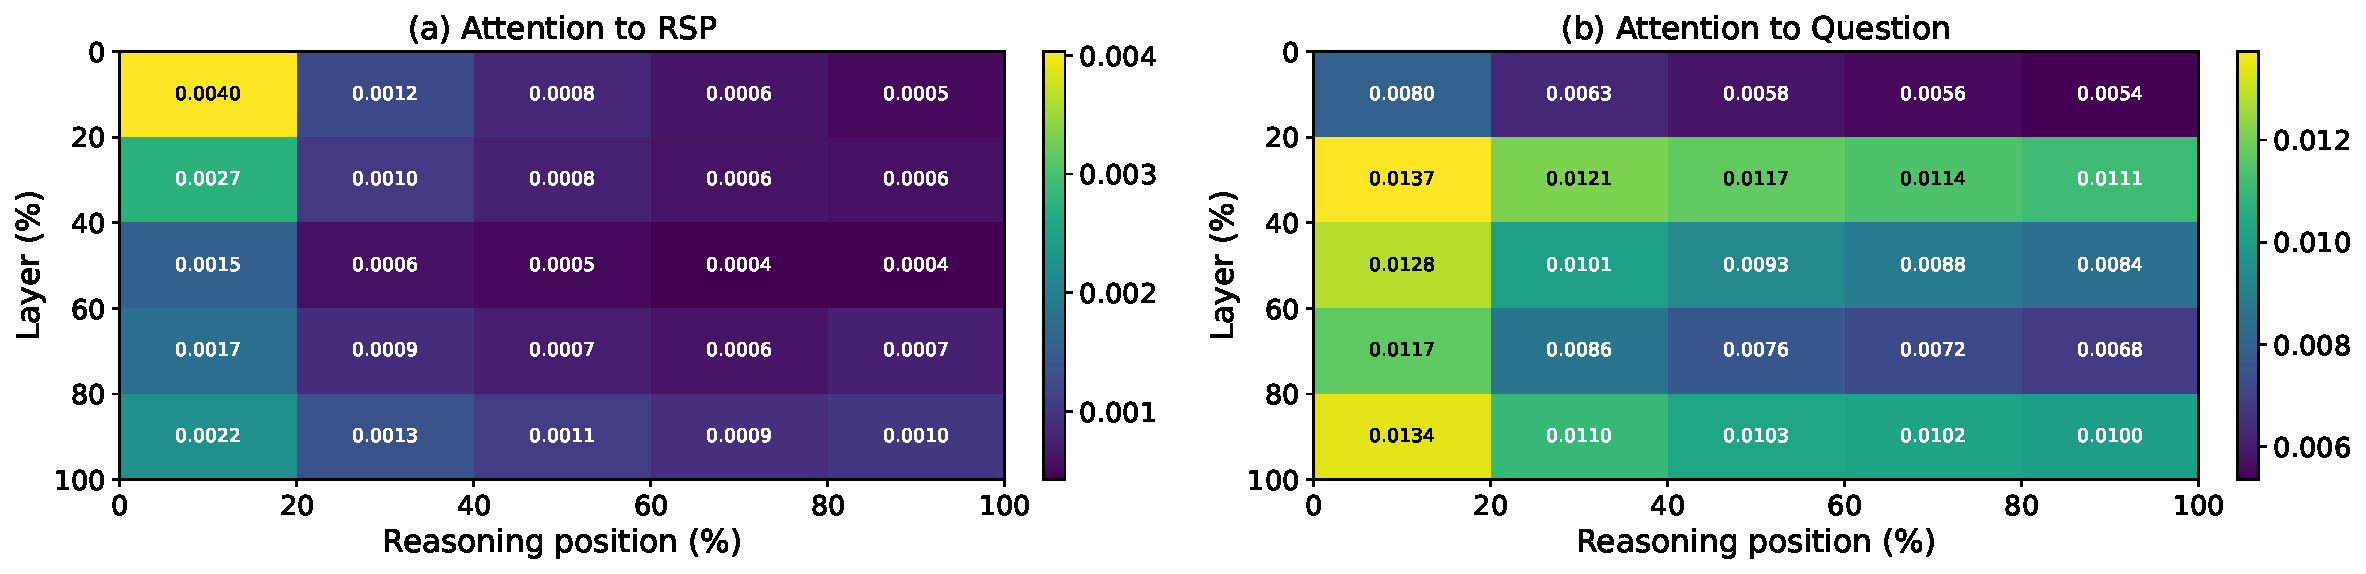
\includegraphics[width=0.72\textwidth]{img/attention/heatmap_qwen7b_suffix.pdf}
  \caption{Qwen2.5-Math-7B의 토큰별 attention 질량(suffix, MATH-500 500문제, 문제마다 독립 RSP). (a) RSP 토큰 attention은 추론 위치 축에서 감소하며 Eq.~\eqref{eq:sandwich}와 맞는다. 레이어 축의 추가 감소는 깊은 레이어가 real-vs-random gap을 더 날카롭게 만든다는 별도 경험적 현상이지, Theorem~\ref{thm:decay}만의 직접 귀결은 아니다. (b) 질문 토큰 attention은 비교적 균일하게 유지된다. 보고한 양은 Appendix~\ref{app:attention_mass}의 per-token mass로, $w_{r,i}^{(\ell)}/L$을 head와 sample에 대해 평균한 값이다.}
  \label{fig:attention_mass}
\end{figure}

% ================================================================
\subsection{성능 향상: 왜 독립 재실행이 도움이 되는가}\label{sec:multipath}
% ================================================================

앞의 두 envelope은 한 rollout 안에서 RSP가 얼마나 움직일 수 있는지를 설명했다. 이제 남는 질문은 성능이다. 왜 \emph{새로운} RSP로 다시 실행할 때, 하나의 고정된 prompt를 반복하는 것보다 이득이 커질 수 있는가? 여기에는 prompt 분포에 대한 사실 하나와, 열린 branch가 실제로 정답에 도움이 되는지에 대한 별도의 task-side 사실 하나가 필요하다.

먼저 분포 쪽 사실부터 보자. 위 attention 항등식과 gap 부등식은 등방성을 요구하지 않지만, branch opening은 현재 prompt에 중요한 방향을 미리 편들지 않는 분포를 선호한다.

\begin{theorem}[방향 무관 미니맥스 커버리지]\label{thm:minimax_directional_coverage}
$\mathbb{R}^d$ 위 평균 0 분포 $D$가 분산 예산 $\mathrm{tr}(\Sigma_D)\le\rho^2$를 만족하면
\[
\min_{\|b\|=1}\mathrm{Var}_{h\sim D}(b^\top h) = \lambda_{\min}(\Sigma_D) \le \rho^2/d
\]
이고, 등호는 $\Sigma_D = (\rho^2/d)\mathbf{I}_d$일 때에만 성립한다.
\end{theorem}

등호에 필요한 핵심은 가우시안 그 자체가 아니라 등방 공분산이다. 여기서 가우시안을 택한 이유는 둘째 성질 때문이다. 가우시안 법칙은 모든 비공집합 열린집합에 양의 확률을 부여하므로, 2차 모멘트 수준에서 특정 방향을 미리 편들지 않으면서도 국소적인 branch-opening 영역을 배제하지 않는다(Proposition~\ref{prop:gaussian_open_support}).

이제 centered prompt $\bar h = 0$ 주변에서 next-token logit의 1차 affine surrogate를
\[
z_i^{\mathrm{lin}}(\bar h) := z_i + a_i^\top \bar h,
\qquad
a_i := \nabla_{\bar h} z_i(0)
\]
로 둔다. baseline에서 제외된 토큰 $i$의 top-$K$ 진입 영역은
\[
\mathcal{G}_{i,K}
\;:=\;
\bigl\{\bar h \in \mathbb{R}^d : \#\{j\neq i : z_j^{\mathrm{lin}}(\bar h) > z_i^{\mathrm{lin}}(\bar h)\} \le K-1\bigr\}
\]
로 쓸 수 있다.

\begin{proposition}[조건부 top-$K$ 진입]\label{prop:support_expansion}
$\mathcal{G}_{i,K}$가 비공집합 열린집합을 포함하면, 등방 가우시안 prompt 법칙이 그 영역에 양의 확률을 부여하므로
\[
\mu_i := \Pr_{\bar h}(\bar h \in \mathcal{G}_{i,K}) > 0
\]
이다.
\end{proposition}

Proposition~\ref{prop:support_expansion}이 설명하는 메커니즘은 의도적으로 제한적이다. branch가 열릴 수 있다는 뜻이지, 열린 branch가 유용하다는 뜻은 아니다. 이를 task accuracy로 연결하려면 task-side 가정을 따로 둬야 한다. 문제 $x$에 대해 (M1) 각 독립 RSP 실행이 정답 trajectory에 도달할 주변 확률이 적어도 $p_{\min}(x)>0$이고, (M2) $N$번의 실행이 서로 독립이라고 하자.

\begin{proposition}[다중 경로 Pass@N]\label{prop:multi_path}
(M1)--(M2) 아래에서, $N$개의 독립 RSP 실행은
\[
\Pr\!\big(\mathrm{Pass@}N\text{ on }x\big) \;\ge\; 1-(1-p_{\min}(x))^N \;\ge\; 1-\exp(-N\,p_{\min}(x))
\]
를 만족한다.
\end{proposition}

이 역할 분담이 이 절의 핵심 해석이다. 메커니즘은 baseline 밖 후보를 \emph{후보권 안으로 들이는 것}까지만 책임진다. 들인 branch가 실제로 \emph{생산적}인지는 task의 성질에 달려 있으므로 $p_{\min}(x)>0$ 가정이 따로 필요하다. 같은 RSP를 모든 sample이 공유하면 누적 이득이 사라지는 이유도 여기 있다. 독립 재추첨이 없으면 branch를 다시 여는 것이 아니라 같은 branch를 반복 방문하게 되기 때문이다. §\ref{sec:experimental_analysis}는 바로 이 서명을 실험적으로 확인한다.

%%%%%%%%%%%%%%%%%%%%%%%%%%%%%%%%
% This file is loaded as Section 4 (empirical) in the new structure.
% Filename retained for git history continuity.
%%%%%%%%%%%%%%%%%%%%%%%%%%%%%%%%

\section{실험적 확인}\label{sec:experimental_analysis}

\S\ref{sec:why_rsp_works}는 세 가지 분리된 메커니즘을 예측한다. RSP는 (i) 출력 분포를 평탄화·재배열해 \emph{token-level} branching을 열고, (ii) 그 branching이 디코딩 동안 의미적으로 다른 \emph{trajectory-level} 궤적으로 propagate되며, (iii) rollout 사이의 독립 재추첨이 그 분기들을 $N$번에 걸쳐 \emph{outcome-level} Pass@$N$으로 누적시킨다. 이 세 예측을 같은 순서로 검증한다. \S\ref{sec:performance}는 RSP가 baseline 정확도를 보존하거나 회복하는 setting을 짚어 메커니즘이 동작할 \emph{대상 영역}을 확정하고, \S\ref{sec:entropy}는 (i)의 첫 측면인 \emph{출력 분포 평탄화}(entropy 상승, top-1 probability 감소, varentropy 증가)가 RSP와 다른 latent prompt 방법에서 공유되는지를 보며, \S\ref{sec:diversity}는 (i)의 두 번째 측면인 \emph{rank-changing} 변화(temperature가 만들 수 없는 순위 재배치), (ii) 의미적 trajectory diversity, (iii) \emph{독립} RSP에서만 누적되는 Pass@$N$을 차례로 검증한다.

% ================================================================
\subsection{실험 설정}\label{sec:setup}
% ================================================================

평가는 세 가지 수학 추론 벤치마크 MATH-500 \citep{lightman2024lets}, GSM8K \citep{cobbe2021training}, AIME24에서 수행한다. 모델은 LLaMA-3.1-8B-Instruct \citep{grattafiori2024llama}와 Qwen2.5-Math 계열 \citep{yang2024qwen25math}을 쓰며, instruct·base·chat template 불일치 base를 비교한다. 모든 실험은 sampling 자체의 무작위성과 RSP 효과를 분리하기 위해 greedy decoding을 사용한다. RSP는 \S\ref{sec:rsp_definition}의 정의를 따르며 기본 \emph{suffix} 위치에 batch마다 새로 추첨된 $\mathbf{H}$를 결합한다. Theorem~\ref{thm:decay}이 RSP 길이 $L$을 최대 섭동 영향력을 정하는 설계 파라미터로 식별하므로, 모델별로 $L \in \{10,15,20\}$를 ablate해 적절한 섭동 강도를 찾는다. Table~\ref{tab:performance}와 Table~\ref{tab:prior_comparison}는 모델별로 선택된 $L$의 결과를 보고한다. \S\ref{sec:entropy}–\S\ref{sec:diversity}의 메커니즘 분석은 fixed $L=10$, \emph{suffix}로 통일해 selection effect에서 분리했다. 전체 설정과 위치별 결과는 Appendix~\ref{app:setup}에 있다.

% ================================================================
\subsection{RSP는 추론 성능을 개선할까?}\label{sec:performance}
% ================================================================

\begin{table}[!t]
\centering
\caption{모델 설정과 벤치마크별 정확도(\%). 괄호 안 값은 baseline 대비 변화량이다. \emph{infix}를 포함한 위치별 전체 결과는 Appendix~\ref{app:ablation}에 있다.}
\label{tab:performance}
\footnotesize
\setlength{\tabcolsep}{3pt}
\renewcommand{\arraystretch}{0.9}
\resizebox{\textwidth}{!}{%
\begin{tabular}{l ccc ccc ccc}
\toprule
 & \multicolumn{3}{c}{\textbf{MATH-500}} & \multicolumn{3}{c}{\textbf{GSM8K}} & \multicolumn{3}{c}{\textbf{AIME24}} \\
\cmidrule(lr){2-4} \cmidrule(lr){5-7} \cmidrule(lr){8-10}
\textbf{Model} & Baseline & \cellcolor{blue!10}RSP(\textit{prefix}) & \cellcolor{blue!10}RSP(\textit{suffix}) & Baseline & \cellcolor{blue!10}RSP(\textit{prefix}) & \cellcolor{blue!10}RSP(\textit{suffix}) & Baseline & \cellcolor{blue!10}RSP(\textit{prefix}) & \cellcolor{blue!10}RSP(\textit{suffix}) \\
\midrule
\multicolumn{10}{l}{\textit{Instruct Models}} \\
\midrule
LLaMA-3.1-8B-Inst      & 52.20 & \cellcolor{blue!10}45.00 {\scriptsize($-$7.2)}  & \cellcolor{blue!10}49.40 {\scriptsize($-$2.8)}  & 85.75 & \cellcolor{blue!10}76.35 {\scriptsize($-$9.4)}  & \cellcolor{blue!10}86.73 {\scriptsize(+1.0)}  & 6.67  & \cellcolor{blue!10}3.33  {\scriptsize($-$3.3)}  & \cellcolor{blue!10}10.00 {\scriptsize(+3.3)}  \\
Qwen2.5-Math-7B-Inst   & 83.20 & \cellcolor{blue!10}81.40 {\scriptsize($-$1.8)}  & \cellcolor{blue!10}83.40 {\scriptsize(+0.2)}    & 95.45 & \cellcolor{blue!10}94.92 {\scriptsize($-$0.5)}  & \cellcolor{blue!10}95.68 {\scriptsize(+0.2)}  & 13.33 & \cellcolor{blue!10}13.33 {\scriptsize(+0.0)}    & \cellcolor{blue!10}16.67 {\scriptsize(+3.3)}  \\
Qwen2.5-Math-1.5B-Inst & 73.00 & \cellcolor{blue!10}74.80 {\scriptsize(+1.8)}    & \cellcolor{blue!10}74.20 {\scriptsize(+1.2)}    & 85.29 & \cellcolor{blue!10}85.29 {\scriptsize(+0.0)}    & \cellcolor{blue!10}84.69 {\scriptsize($-$0.6)} & 10.00 & \cellcolor{blue!10}13.33 {\scriptsize(+3.3)}    & \cellcolor{blue!10}20.00 {\scriptsize(+10.0)} \\
\midrule
\multicolumn{10}{l}{\textit{Base Models (Raw Text)}} \\
\midrule
Qwen2.5-Math-7B        & 72.20 & \cellcolor{blue!10}71.60 {\scriptsize($-$0.6)}  & \cellcolor{blue!10}55.60 {\scriptsize($-$16.6)} & 84.15 & \cellcolor{blue!10}84.31 {\scriptsize(+0.2)}    & \cellcolor{blue!10}54.13 {\scriptsize($-$30.0)} & 6.67  & \cellcolor{blue!10}16.67 {\scriptsize(+10.0)}   & \cellcolor{blue!10}13.33 {\scriptsize(+6.7)}  \\
Qwen2.5-Math-1.5B      & 61.40 & \cellcolor{blue!10}64.40 {\scriptsize(+3.0)}    & \cellcolor{blue!10}54.60 {\scriptsize($-$6.8)}  & 77.86 & \cellcolor{blue!10}74.30 {\scriptsize($-$3.6)}  & \cellcolor{blue!10}58.61 {\scriptsize($-$19.3)} & 16.67 & \cellcolor{blue!10}10.00 {\scriptsize($-$6.7)}  & \cellcolor{blue!10}3.33  {\scriptsize($-$13.3)} \\
\midrule
\multicolumn{10}{l}{\textit{Base Models + ChatML (Format Mismatch)}} \\
\midrule
Qwen2.5-Math-7B        & 52.20 & \cellcolor{blue!10}59.20 {\scriptsize(+7.0)}    & \cellcolor{blue!10}70.40 {\scriptsize(+18.2)}   & 58.30 & \cellcolor{blue!10}56.41 {\scriptsize($-$1.9)}  & \cellcolor{blue!10}75.97 {\scriptsize(+17.7)} & 23.33 & \cellcolor{blue!10}3.33  {\scriptsize($-$20.0)} & \cellcolor{blue!10}23.33 {\scriptsize(+0.0)}  \\
Qwen2.5-Math-1.5B      & 34.40 & \cellcolor{blue!10}63.40 {\scriptsize(+29.0)}   & \cellcolor{blue!10}51.00 {\scriptsize(+16.6)}   & 37.45 & \cellcolor{blue!10}67.02 {\scriptsize(+29.6)}   & \cellcolor{blue!10}50.64 {\scriptsize(+13.2)} & 13.33 & \cellcolor{blue!10}20.00 {\scriptsize(+6.7)}    & \cellcolor{blue!10}13.33 {\scriptsize(+0.0)}  \\
\bottomrule
\end{tabular}}
\end{table}

먼저 무작위 임베딩 주입이 추론 성능에 어떤 영향을 주는지 본다. Table~\ref{tab:performance}는 기본 \emph{suffix} 위치와 \emph{prefix} ablation 결과를 보고한다.

instruct model에서 RSP는 baseline 대비 ±몇 \%p 안에서 거동한다. 가장 두드러지는 것은 형식 불일치 회복이다. chat 형식으로 학습되지 않은 base model에 ChatML template을 적용하면 \emph{Suffix}(Qwen2.5-Math-7B에서 +18.2/+17.7\,pp)와 \emph{prefix}(Qwen2.5-Math-1.5B에서 +29.0/+29.6\,pp까지)가 손실을 회복한다 --- 단순 노이즈였다면 추가 저하가 나타나야 한다. 한편 base raw-text 환경에서 \emph{suffix}는 큰 손해를 보이고($-$16.6/$-$30.0\,pp) \emph{prefix}는 손실이 작은데, base가 EOS 인접 신호를 탈선 trigger로 처리하고 \emph{prefix}가 그것을 회피한다고 볼 수 있다. 즉 RSP의 직접적 정확도 이득은 misaligned 입력 회복에 집중되고 잘 정렬된 instruct에서는 ±몇 pp에 머문다. 본 논문이 강조하는 효과는 \S\ref{sec:diversity}의 token·trajectory·outcome diversity이고, 정확도 회복은 부수적 결과다.

\begin{table}[!t]
\centering
\caption{기존 soft prompt 방법(TTSV, SoftCoT, LTPO)과의 통합 평가 비교. \textbf{Baseline}은 Table~\ref{tab:performance}에서 가져왔고, \textbf{RSP}는 평가셋에서 위치 및 $L\in\{10,15,20\}$에 대한 best 값을 보고한다(위치별 분해는 Appendix~\ref{app:ablation}). \textbf{Bold}는 최고 성능, \underline{underline}은 두 번째 성능이다.}
\label{tab:prior_comparison}
\footnotesize
\renewcommand{\arraystretch}{0.9}
\begin{tabular}{llccccc}
\toprule
\textbf{Model} & \textbf{Benchmark} & \textbf{Baseline} & \cellcolor{blue!10}\textbf{RSP} & \textbf{TTSV} & \textbf{SoftCoT} & \textbf{LTPO} \\
\midrule
\multirow{3}{*}{Qwen2.5-Math-7B-Instruct} & MATH-500 & 83.20 & \cellcolor{blue!10}\textbf{84.20} & \underline{83.80} & 82.80 & 83.00 \\
 & GSM8K   & \underline{95.45} & \cellcolor{blue!10}\textbf{95.68} & 95.30 & 95.00 & 94.84 \\
 & AIME24  & 13.33 & \cellcolor{blue!10}\underline{16.67} & \textbf{23.30} & \underline{16.67} & 13.33 \\
\midrule
\multirow{3}{*}{Qwen2.5-Math-1.5B-Instruct} & MATH-500 & 73.00 & \cellcolor{blue!10}\underline{75.20} & \underline{75.20} & \textbf{76.00} & 72.40 \\
 & GSM8K   & 85.29 & \cellcolor{blue!10}\textbf{85.75} & \underline{85.70} & 84.46 & 84.53 \\
 & AIME24  & \underline{10.00} & \cellcolor{blue!10}\textbf{20.00} &  6.70 &  6.67 & \underline{10.00} \\
\bottomrule
\end{tabular}
\end{table}

또한 RSP를 TTSV, SoftCoT, LTPO처럼 서로 다른 목적 함수로 임베딩을 최적화하는 기존 soft prompt 방법과 비교했다. Table~\ref{tab:prior_comparison}은 공통 answer extraction pipeline(Appendix~\ref{app:extraction}) 아래에서 다시 평가한 결과를 보여 준다. 각 방법은 프롬프트 형식과 채점 규칙이 다르지만, fallback 기반 추출로 형식 민감도를 낮춘 비교를 수행했다. RSP는 일관된 우월성을 보이지 않는다. 예컨대 Qwen2.5-Math-7B-Inst의 AIME24에서 TTSV가 23.30\%로 RSP의 16.67\%를 앞선다. 그러나 RSP가 \emph{추가 학습 없이도} 학습 기반 방법과 비교 가능한 범위에 도달한다는 사실 자체가, soft prompt 효과의 일정 부분이 학습된 의미가 아니라 \emph{주입 구조}에서 비롯될 수 있음을 가리키는 본 논문의 주된 증거가 된다.

% ================================================================
\subsection{RSP는 출력 분포를 어떻게 바꾸는가?}\label{sec:entropy}
% ================================================================

다음으로 RSP 주입이 생성 과정의 출력 분포를 어떻게 바꾸는지 살펴본다. 설정은 Qwen2.5-Math-1.5B-Instruct와 MATH-500이며, 토큰별 entropy, top-1 probability, varentropy를 생성 단계에 따라 측정한다. Figure~\ref{fig:entropy_first5}는 생성 초반 5\% 구간에서 RSP 변형과 기존 soft prompt 방법을 비교한 결과이며, 전체 곡선은 Appendix~\ref{app:entropy_full}에 있다.

\begin{figure}[ht]
  \centering
  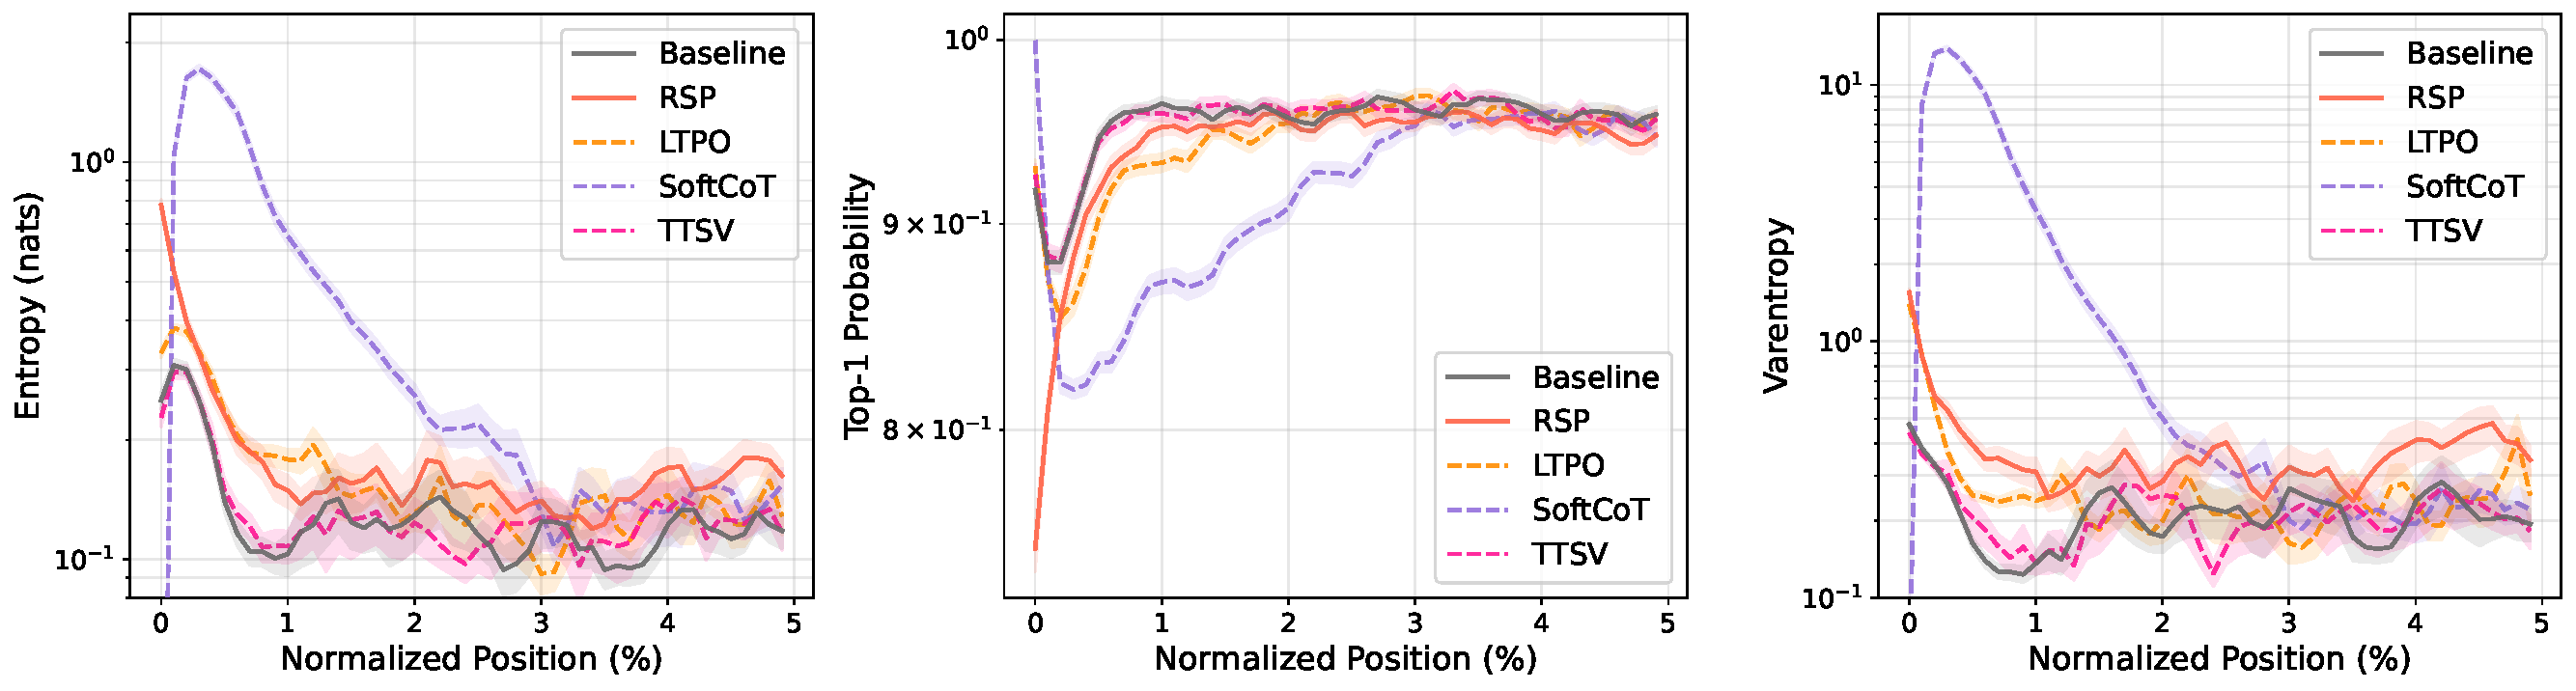
\includegraphics[width=\textwidth]{img/entropy/entropy_first5pct_zoom.pdf}
  \caption{생성 초반 5\% 구간의 평균 entropy, top-1 probability, varentropy (Qwen2.5-Math-1.5B-Instruct, MATH-500). 음영은 $\pm$1 SEM이다. 실선은 RSP 변형과 baseline, 점선은 기존 soft prompt 방법(LTPO, SoftCoT, TTSV)이다.}
  \label{fig:entropy_first5}
\end{figure}

RSP를 포함한 latent prompt 방법들은 공통적으로 \emph{생성 초반 entropy 상승 → 후반 baseline 수렴}이라는 동일한 시그니처를 보인다. 메커니즘 측면에서 자연스러운 설명은 OOV(out-of-vocabulary) 효과다 --- 어휘 바깥의 연속 임베딩이 입력으로 들어오면 모델은 익숙한 토큰 분포 위에서 한 번도 본 적 없는 키 위치를 attend해야 하므로 초반 next-token 분포에서 확률 질량이 여러 후보로 재분배된다. 세 RSP 주입 위치 모두에서 초반 entropy↑, top-1 probability↓, varentropy↑가 함께 나타나며, 이는 multimodal 분포와 정합한다 \citep{ahmed2026logitscope}. 변화가 생성 초반에 국한되고 중·후반에는 세 지표 모두 baseline 수준으로 수렴한다는 점이 중요한데, 이는 \S\ref{sec:converge}의 cache-growth attenuation이 예측한 \emph{초반 영향력 → 캐시 성장에 따른 자동 감쇠} 패턴과 정합한다.

서로 다른 목적 함수로 학습된 prior 방법(LTPO, SoftCoT, TTSV)도 같은 시그니처를 공유한다. 평균 entropy를 \emph{줄이는} 보상을 쓰는 TTSV조차 초반 구간만큼은 baseline과 비슷하다. entropy 수치 자체가 quality score가 아닌 점은 짚어 둘 만하다 --- 높은 entropy가 무조건 좋은 것이 아니라, 시그니처가 드러내는 것은 학습 목적과 무관하게 OOV 임베딩 주입이 같은 fingerprint를 만든다는 \emph{공유 메커니즘}이다. latent reasoning을 가능케 하는 핵심 요소가 학습된 의미가 아니라 \emph{주입 자체}에 있다는 가설을 이 시그니처가 뒷받침한다.

% ================================================================
\subsection{RSP는 실제로 추론 궤적의 다양성을 만드는가?}\label{sec:diversity}
% ================================================================

\S\ref{sec:entropy}는 RSP가 생성 초반 출력 분포를 바꾼다는 사실을 보였다. 이제 이 변화가 실제 추론 다양성으로 이어지는지를 세 수준에서 살펴본다. 분석 수준은 토큰 순위, 궤적의 의미적 내용, 과제 수준 결과다. 세 분석 모두 Qwen2.5-Math-1.5B-Instruct, MATH-500, \emph{suffix} 주입, $L=10$ 설정을 공유한다.

\paragraph{토큰 수준: temperature를 넘어서는 분포 변화.}
\begin{wraptable}{r}{0.55\textwidth}
  \vspace{-1.2em}
  \centering
  \caption{Baseline $\tau{=}1.0$을 기준으로 본 첫 토큰 분포 지표. 더 높은 temperature의 baseline($\tau{=}2.0,3.0$)과 RSP $\tau{=}1.0$을 비교한다. RSP 지표는 16개 random seed 평균이며, Acc는 문제당 16개 샘플의 평균 $\pm$ 표준편차다.}
  \label{tab:rsp_vs_temp}
  \footnotesize
  \setlength{\tabcolsep}{3.5pt}
  \renewcommand{\arraystretch}{0.9}
  \begin{tabular}{lccc}
    \toprule
    \textbf{Metric} & \textbf{$\tau{=}2.0$} & \textbf{$\tau{=}3.0$} & \cellcolor{blue!10}\textbf{RSP} \\
    \midrule
    Spearman $\rho$ & 1.000 & 1.000 & \cellcolor{blue!10}\textbf{0.709} \\
    Mass outside top-10 & 5.18\% & 29.11\% & \cellcolor{blue!10}\textbf{21.86\%} \\
    JS divergence & 0.060 & 0.218 & \cellcolor{blue!10}\textbf{0.131} \\
    Acc (\%) & 20.77 $\pm$ 1.47 & 1.42 $\pm$ 0.35 & \cellcolor{blue!10}\textbf{73.30 $\pm$ 1.07} \\
    \bottomrule
  \end{tabular}
\end{wraptable}
RSP가 첫 토큰 분포를 얼마나 흔드는지를 정량화한다 --- 추론 궤적의 분기점이다 \citep{wang2025beyond}. Baseline $\tau{=}1.0$을 기준으로, 더 높은 temperature($\tau{=}2.0,3.0$, 문제당 16개 샘플)과 RSP $\tau{=}1.0$(16 seed 평균)을 세 지표로 비교한다: 순위 재배치를 감지하는 Spearman rank correlation $\rho$, support 확장을 측정하는 baseline top-10 밖 확률 질량, 전체 분포 변화 크기를 정량화하는 Jensen--Shannon divergence (정식 정의는 Appendix~\ref{app:token_metrics}). Table~\ref{tab:rsp_vs_temp}의 대비는 명확하다. RSP의 분포 변화 크기는 $\tau{=}2.0$과 $\tau{=}3.0$ 사이지만 메커니즘이 다르다 --- temperature는 단조 변환이라 $\rho=1$이 강제되는 반면 RSP는 $\rho=0.709$로 순위를 일부 보존하면서 재배치한다. Pass@1 행이 비용을 드러낸다 --- temperature를 RSP와 같은 크기로 키우면 정확도는 1.42\%까지 무너지지만 RSP는 73.30\%를 유지한다. 따라서 RSP는 temperature와 근본적으로 다른 섭동을 만든다. 또한 RSP의 16 seed 정확도 변동성($\pm 1.07$)은 $\tau{=}2.0$ 16 샘플의 변동성($\pm 1.47$)과 비교 가능한 수준이다.

\paragraph{궤적 수준: 의미적 다양성.}
\begin{wraptable}{r}{0.34\textwidth}
  \vspace{-1.2em}
  \centering
  \caption{64개 문제에 대해 평균한 의미적 다양성 지표.}
  \label{tab:semantic_metrics}
  \footnotesize
  \setlength{\tabcolsep}{4pt}
  \renewcommand{\arraystretch}{0.9}
  \begin{tabular}{lcc}
    \toprule
    \textbf{Metric} & \textbf{Baseline} & \cellcolor{blue!10}\textbf{RSP} \\
    \midrule
    Pairwise cos.\ dist. & 0.0612 & \cellcolor{blue!10}\textbf{0.0879} \\
    Inter-cluster dist. & 0.0183 & \cellcolor{blue!10}\textbf{0.0982} \\
    Intra-cluster dist. & 0.0526 & \cellcolor{blue!10}0.0528 \\
    \bottomrule
  \end{tabular}
\end{wraptable}
토큰 수준 재배치는 두 번째 질문을 만든다 --- 첫 토큰 섭동이 서로 \emph{다른} 궤적으로 갈라지는가, 아니면 비슷한 궤적으로 수렴하는가? MATH-500에서 무작위 64개 문제를 뽑고, Baseline과 RSP 두 조건에서 각 문제마다 $\tau{=}1.0$으로 300개의 독립 궤적을 생성했다. 각 궤적을 BGE-M3 \citep{chen2024bge}로 임베딩하고 세 지표를 계산한다 --- 의미적 spread 전체를 보는 \textit{pairwise cosine distance}, density 기반 클러스터링 알고리즘인 DBSCAN \citep{ester1996density} 군집 중심 사이의 \textit{inter-cluster distance}(서로 다른 궤적 그룹의 분리), 그리고 군집 내 응집을 보는 \textit{intra-cluster distance}. Table~\ref{tab:semantic_metrics}는 세 패턴을 동시에 드러낸다 --- pairwise cosine distance가 1.4배로 커지고, inter-cluster distance가 5.4배로 뛰며, intra-cluster distance는 거의 변하지 않는다. 즉 궤적 집합이 더 다양해지고 더 분리된 군집들로 갈라지면서도 군집 내부 응집은 유지된다. RSP는 pairwise distance 기준으로도 64개 중 56개 문제에서 baseline보다 컸다.

\paragraph{결과 수준: Pass@$N$ 스케일링.}
마지막 결과 수준에서는, 이러한 다양성이 실제 과제 성과로 이어지는지를 Pass@$N$ \citep{chen2021codex}로 본다($N$개 샘플 중 적어도 하나가 정답일 확률). MATH-500과 AIME24에서 문제당 16개 샘플을 생성하고 네 조건을 비교한다 --- \textit{(i)} \textit{Baseline} + $\tau{=}1.0$, \textit{(ii)} \textit{RSP (single seed)} + $\tau{=}1.0$, 모든 샘플이 같은 RSP 공유, \textit{(iii)} \textit{RSP (indep.\ seed)} + greedy, 샘플마다 새 RSP, \textit{(iv)} \textit{RSP (indep.\ seed)} + $\tau{=}1.0$, 샘플마다 새 RSP.

\begin{figure}[ht]
  \centering
  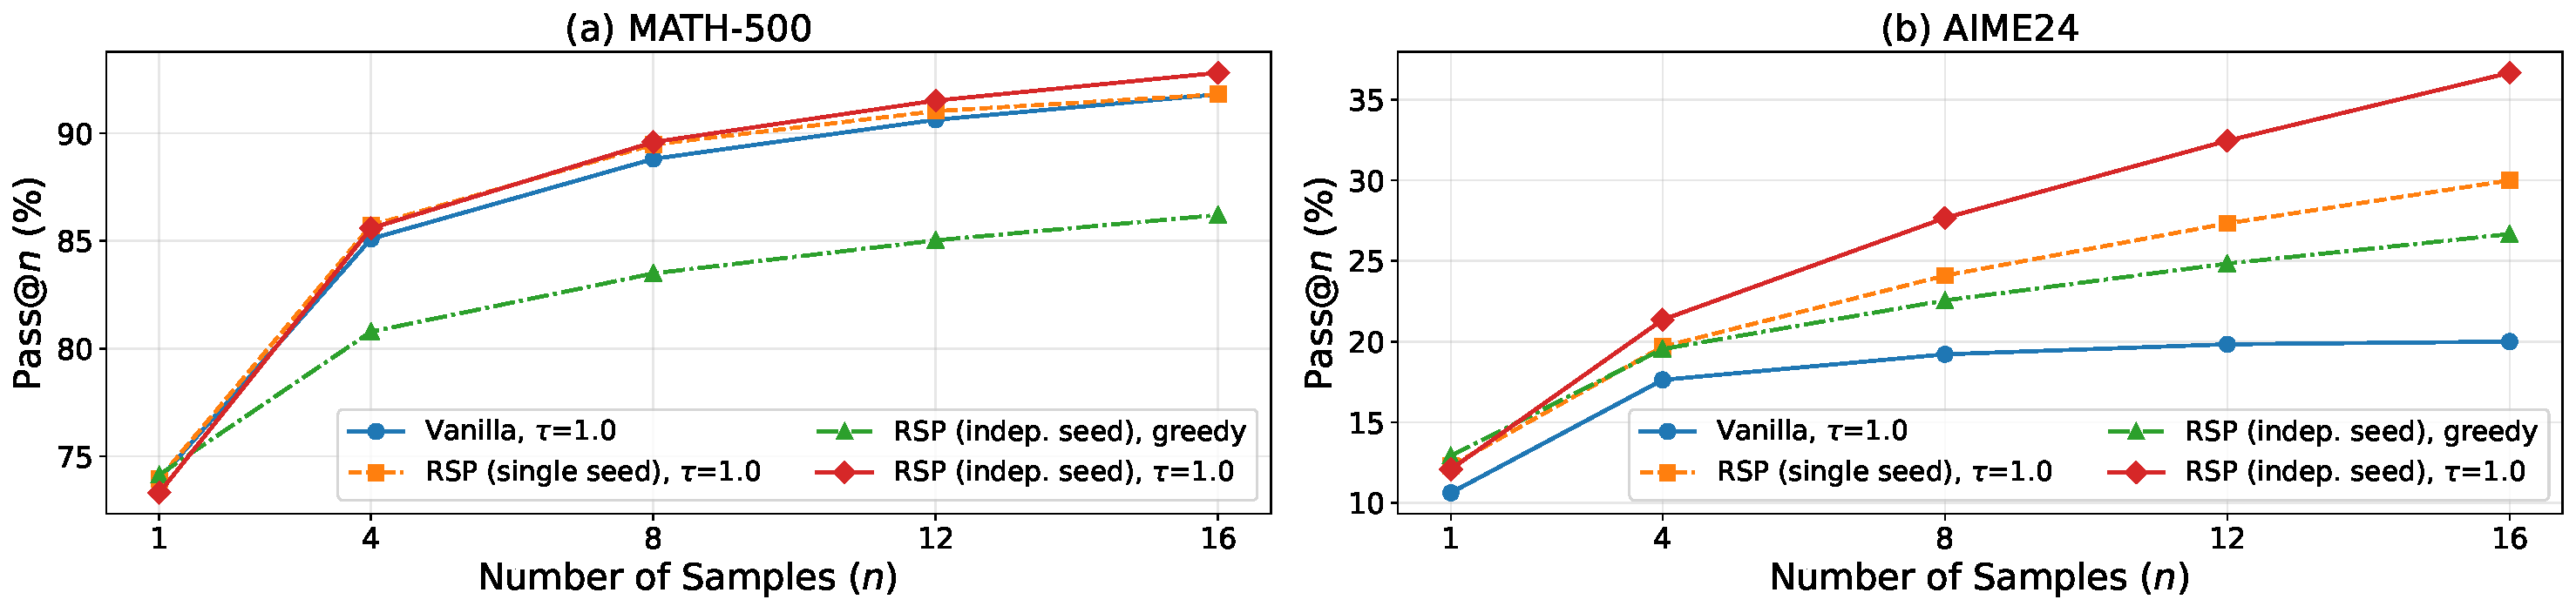
\includegraphics[width=0.9\textwidth]{img/diversity/pass_at_n_combined.pdf}
  \caption{Qwen2.5-Math-1.5B-Instruct에서의 Pass@$N$ 스케일링. 좌측은 MATH-500, 우측은 AIME24이며, 문제당 16개 샘플 사용. \textit{Baseline}: temperature sampling만. \textit{RSP (single seed)}: 고정된 하나의 RSP와 temperature를 함께. \textit{RSP (indep.\ seed)}: 샘플마다 다른 RSP를 쓰는 경우(temperature 유무).}
  \label{fig:pass_at_n}
\end{figure}

조건 \textit{(iv)}가 두 벤치마크 모두에서 가장 높은 Pass@$N$을 달성하며 $N=16$에서 MATH-500 92.80\%, AIME24 36.67\%에 이른다. \textit{(ii)}는 baseline 대비 거의 개선이 없어, 다양성 이득의 핵심이 \emph{고정} 섭동이 아니라 샘플마다 \emph{독립}된 무작위 임베딩임을 드러낸다. Pass@1은 MATH-500에서 baseline 수준을 유지하고 더 어려운 AIME24에서는 \textit{(iv)}가 더 높아, 독립 RSP + temperature 결합이 단일 샘플 정확도를 해치지 않으면서 추론 궤적을 다양화한다.

%%%%%%%%%%%%%%%%%%%%%%%%%%%%%%%%
% Chapter 5. Conclusion
%%%%%%%%%%%%%%%%%%%%%%%%%%%%%%%%

\section{결론}\label{sec:conclusion}

본 논문은 사전학습 임베딩 행렬의 항별 통계에 맞춘 등방 가우시안에서 추첨한 RSP가 학습 없이도 영향을 줄 수 있는 이유를 transformer 수준에서 분석했다. 분석의 핵심은 네 가지다. exact attention decomposition, 초반 exploration의 lower envelope(§\ref{sec:improve}), 후반 감쇠의 upper envelope(§\ref{sec:converge}), 그리고 독립 재추첨과 별도의 과제 측 성공 가정이 더해질 때에만 Pass@$N$ 증가로 이어지는 branch-opening 논리(§\ref{sec:multipath})다. §\ref{sec:experimental_analysis}의 실험은 이 구조와 맞물린다. 학습 없는 RSP는 경쟁적인 성능을 유지하고, 초반 토큰 분포는 더 다양해진 뒤 후반에 안정화되며, 같은 RSP를 모든 sample에 공유하면 누적 이득이 사라진다. RSP는 순위를 \emph{바꾸는} 섭동이고 temperature는 순위를 \emph{보존}하는 섭동이므로 둘은 직교적이며, 이는 GRPO \citep{shao2024deepseekmath}의 entropy collapse를 DAPO \citep{yu2025dapo}, CE-GPPO \citep{su2025cegppo} 너머에서 샘플링 단계로 보완할 가능성을 시사한다. RSP를 활용한 학습 시점 비교, 수학 추론을 넘어선 도메인 확장, RSP 길이·주입 위치의 원리적 결정은 향후 과제다.


\bibliographystyle{plainnat}
\bibliography{biblist}

\appendix

%%%%%%%%%%%%%%%%%%%%%%%%%%%%%%%%%%%%%%%%%%%%%%%%
% Appendix
%%%%%%%%%%%%%%%%%%%%%%%%%%%%%%%%%%%%%%%%%%%%%%%%

\clearpage
\section{실험 설정과 전체 정확도 분석}\label{app:setup}\label{app:ablation}

Table~\ref{tab:performance_full}은 본문 Table~\ref{tab:performance}에서 위치별 최고 성능만 요약해 제시한 결과를, Prefix, Infix, Suffix별 전체 정확도로 다시 펼쳐 보인다. Table~\ref{tab:token_count}는 각 모델--벤치마크 조합에서 사용한 RSP 토큰 수 $L$을 정리한 것으로, 후보 집합 $\{10, 15, 20\}$에서 선택했다. 모든 실험은 단일 NVIDIA A6000 40GB GPU에서 greedy decoding으로 수행했으며, 최대 생성 길이는 MATH-500과 GSM8K에서 3{,}072 토큰, AIME24에서 4{,}096 토큰으로 고정했다. 배치 크기는 모델별로 고정했다(LLaMA-3.1-8B-Instruct와 Qwen2.5-Math-7B 계열은 16, Qwen2.5-Math-1.5B 계열은 32).

\begin{table}[ht]
\centering
\caption{모델 설정, 주입 위치, 벤치마크별 정확도(\%). 괄호 안 값은 baseline 대비 변화량이다. \textbf{굵게}는 최고 성능, \underline{밑줄}은 각 모델--벤치마크 조합에서 두 번째 성능을 뜻한다.}
\label{tab:performance_full}
\footnotesize
\renewcommand{\arraystretch}{0.9}
\begin{tabular}{ll ccc}
\toprule
\textbf{Model} & \textbf{Mode} & \textbf{MATH-500} & \textbf{GSM8K} & \textbf{AIME24} \\
\midrule
\multicolumn{5}{l}{\textit{Instruct Models}} \\
\midrule
\multirow{4}{*}{LLaMA-3.1-8B-Instruct} & Baseline & \textbf{52.20} & 85.75 & \underline{6.67} \\
 & Prefix & 45.00 {\scriptsize($-$7.2)} & 76.35 {\scriptsize($-$9.4)} & 3.33 {\scriptsize($-$3.3)} \\
 & Infix & \underline{49.40} {\scriptsize($-$2.8)} & \underline{85.97} {\scriptsize(+0.2)} & \textbf{10.00} {\scriptsize(+3.3)} \\
 & Suffix & \underline{49.40} {\scriptsize($-$2.8)} & \textbf{86.73} {\scriptsize(+1.0)} & \textbf{10.00} {\scriptsize(+3.3)} \\
\midrule
\multirow{4}{*}{Qwen2.5-Math-7B-Instruct} & Baseline & 83.20 & 95.45 & \underline{13.33} \\
 & Prefix & 81.40 {\scriptsize($-$1.8)} & 94.92 {\scriptsize($-$0.5)} & \underline{13.33} {\scriptsize(+0.0)} \\
 & Infix & \textbf{84.20} {\scriptsize(+1.0)} & \underline{95.60} {\scriptsize(+0.2)} & \textbf{16.67} {\scriptsize(+3.3)} \\
 & Suffix & \underline{83.40} {\scriptsize(+0.2)} & \textbf{95.68} {\scriptsize(+0.2)} & \textbf{16.67} {\scriptsize(+3.3)} \\
\midrule
\multirow{4}{*}{Qwen2.5-Math-1.5B-Instruct} & Baseline & 73.00 & \underline{85.29} & 10.00 \\
 & Prefix & \underline{74.80} {\scriptsize(+1.8)} & \underline{85.29} {\scriptsize(+0.0)} & \underline{13.33} {\scriptsize(+3.3)} \\
 & Infix & \textbf{75.20} {\scriptsize(+2.2)} & \textbf{85.75} {\scriptsize(+0.5)} & 6.67 {\scriptsize($-$3.3)} \\
 & Suffix & 74.20 {\scriptsize(+1.2)} & 84.69 {\scriptsize($-$0.6)} & \textbf{20.00} {\scriptsize(+10.0)} \\
\midrule
\multicolumn{5}{l}{\textit{Base Models (Raw Text)}} \\
\midrule
\multirow{4}{*}{Qwen2.5-Math-7B} & Baseline & \textbf{72.20} & \underline{84.15} & 6.67 \\
 & Prefix & \underline{71.60} {\scriptsize($-$0.6)} & \textbf{84.31} {\scriptsize(+0.2)} & \textbf{16.67} {\scriptsize(+10.0)} \\
 & Infix & 63.20 {\scriptsize($-$9.0)} & 64.29 {\scriptsize($-$19.9)} & \textbf{16.67} {\scriptsize(+10.0)} \\
 & Suffix & 55.60 {\scriptsize($-$16.6)} & 54.13 {\scriptsize($-$30.0)} & \underline{13.33} {\scriptsize(+6.7)} \\
\midrule
\multirow{4}{*}{Qwen2.5-Math-1.5B} & Baseline & \underline{61.40} & \textbf{77.86} & \textbf{16.67} \\
 & Prefix & \textbf{64.40} {\scriptsize(+3.0)} & \underline{74.30} {\scriptsize($-$3.6)} & \underline{10.00} {\scriptsize($-$6.7)} \\
 & Infix & 63.20 {\scriptsize(+1.8)} & 73.92 {\scriptsize($-$3.9)} & \underline{10.00} {\scriptsize($-$6.7)} \\
 & Suffix & 54.60 {\scriptsize($-$6.8)} & 58.61 {\scriptsize($-$19.3)} & 3.33 {\scriptsize($-$13.3)} \\
\midrule
\multicolumn{5}{l}{\textit{Base Models + ChatML (Format Mismatch)}} \\
\midrule
\multirow{4}{*}{Qwen2.5-Math-7B} & Baseline & 52.20 & 58.30 & \textbf{23.33} \\
 & Prefix & 59.20 {\scriptsize(+7.0)} & 56.41 {\scriptsize($-$1.9)} & \underline{3.33} {\scriptsize($-$20.0)} \\
 & Infix & \underline{62.00} {\scriptsize(+9.8)} & \underline{69.07} {\scriptsize(+10.8)} & \textbf{23.33} {\scriptsize(+0.0)} \\
 & Suffix & \textbf{70.40} {\scriptsize(+18.2)} & \textbf{75.97} {\scriptsize(+17.7)} & \textbf{23.33} {\scriptsize(+0.0)} \\
\midrule
\multirow{4}{*}{Qwen2.5-Math-1.5B} & Baseline & 34.40 & 37.45 & \underline{13.33} \\
 & Prefix & \textbf{63.40} {\scriptsize(+29.0)} & \textbf{67.02} {\scriptsize(+29.6)} & \textbf{20.00} {\scriptsize(+6.7)} \\
 & Infix & 39.20 {\scriptsize(+4.8)} & 50.42 {\scriptsize(+13.0)} & 6.67 {\scriptsize($-$6.7)} \\
 & Suffix & \underline{51.00} {\scriptsize(+16.6)} & \underline{50.64} {\scriptsize(+13.2)} & \underline{13.33} {\scriptsize(+0.0)} \\
\bottomrule
\end{tabular}
\end{table}

\begin{table}[ht]
\centering
\caption{각 모델과 벤치마크에 사용한 RSP 토큰 수($L$).}
\label{tab:token_count}
\footnotesize
\renewcommand{\arraystretch}{0.9}
\begin{tabular}{lccc}
\toprule
\textbf{Model} & \textbf{MATH-500} & \textbf{GSM8K} & \textbf{AIME24} \\
\midrule
LLaMA-3.1-8B-Instruct & 15 & 20 & 15 \\
Qwen2.5-Math-7B-Instruct & 20 & 20 & 20 \\
Qwen2.5-Math-1.5B-Instruct & 20 & 10 & 20 \\
Qwen2.5-Math-7B & 10 & 10 & 20 \\
Qwen2.5-Math-1.5B & 10 & 10 & 20 \\
Qwen2.5-Math-1.5B (ChatML) & 20 & 20 & 10 \\
Qwen2.5-Math-7B (ChatML) & 20 & 20 & 20 \\
\bottomrule
\end{tabular}
\end{table}

% ================================================================
\subsection{RSP 주입 위치와 프롬프트 템플릿}\label{app:injection_positions}
% ================================================================

아래에는 모든 모델 유형에서 주입 위치별 프롬프트 구조를 정리했다. \textcolor{blue!70!black}{파란색 텍스트}는 RSP 임베딩, \textcolor{purple}{보라색 텍스트}는 특수 토큰을 뜻한다.

% --------------------------------
\subsubsection{Prefix}
% --------------------------------

Prefix 주입에서는 RSP 임베딩을 프롬프트 임베딩 앞에 연결한다. 텍스트 자체는 수정하지 않는다.

\paragraph{ChatML (Qwen Instruct / Base + ChatML).}
\begin{tcolorbox}[colback=gray!5, colframe=black!60, arc=3pt, boxrule=0.5pt, fontupper=\footnotesize\ttfamily, breakable]
\textcolor{blue!70!black}{[Random Embeddings ($L$ tokens)]}\\
\textcolor{purple}{<|im\_start|>}system\\
Please reason step by step, and put your final answer within \textbackslash boxed\{\}.\textcolor{purple}{<|im\_end|>}\\
\textcolor{purple}{<|im\_start|>}user\\
\{question\}\textcolor{purple}{<|im\_end|>}\\
\textcolor{purple}{<|im\_start|>}assistant
\end{tcolorbox}

\paragraph{LLaMA Chat Template.}
\begin{tcolorbox}[colback=gray!5, colframe=black!60, arc=3pt, boxrule=0.5pt, fontupper=\footnotesize\ttfamily, breakable]
\textcolor{blue!70!black}{[Random Embeddings ($L$ tokens)]}\\
\textcolor{purple}{<|begin\_of\_text|>}\\
\textcolor{purple}{<|start\_header\_id|>}system\textcolor{purple}{<|end\_header\_id|>}\\
Cutting Knowledge Date: December 2023\\
Today Date: 26 Jul 2024\\
Please reason step by step, and put your final answer within \textbackslash boxed\{\}.\textcolor{purple}{<|eot\_id|>}\\
\textcolor{purple}{<|start\_header\_id|>}user\textcolor{purple}{<|end\_header\_id|>}\\
\{question\}\textcolor{purple}{<|eot\_id|>}\\
\textcolor{purple}{<|start\_header\_id|>}assistant\textcolor{purple}{<|end\_header\_id|>}
\end{tcolorbox}

\paragraph{Raw Text (Qwen Base).}
\begin{tcolorbox}[colback=gray!5, colframe=black!60, arc=3pt, boxrule=0.5pt, fontupper=\footnotesize\ttfamily, breakable]
\textcolor{blue!70!black}{[Random Embeddings ($L$ tokens)]}\\
\{question\}\\
Please reason step by step, and put your final answer within \textbackslash boxed\{\}.
\end{tcolorbox}

% --------------------------------
\subsubsection{Infix}
% --------------------------------

Infix 주입에서는 설명 문구와 특수 토큰을 프롬프트 내부에 넣은 뒤, 그 특수 토큰 위치를 임베딩 수준에서 RSP로 교체한다.

\paragraph{ChatML (Qwen Instruct / Base + ChatML).}
\begin{tcolorbox}[colback=gray!5, colframe=black!60, arc=3pt, boxrule=0.5pt, fontupper=\footnotesize\ttfamily, breakable]
\textcolor{purple}{<|im\_start|>}system\\
Please reason step by step, and put your final answer within \textbackslash boxed\{\}.\textcolor{purple}{<|im\_end|>}\\
\textcolor{purple}{<|im\_start|>}user\\
\{question\}\\[0.3em]
\textcolor{gray}{There are \{$L$\} special tokens that contain compressed latent reasoning information that might be useful for your reasoning. If these tokens are useful for your case, you can use them as reference. If these tokens are not useful for your case, you can ignore them and focus back to solving the problem.}\\[0.3em]
Here are the \{$L$\} special tokens: \textcolor{blue!70!black}{<special\_token\_1>...<special\_token\_$L$>}\\
\textcolor{purple}{<|im\_end|>}\\
\textcolor{purple}{<|im\_start|>}assistant
\end{tcolorbox}

\paragraph{LLaMA Chat Template.}
\begin{tcolorbox}[colback=gray!5, colframe=black!60, arc=3pt, boxrule=0.5pt, fontupper=\footnotesize\ttfamily, breakable]
\textcolor{purple}{<|begin\_of\_text|>}\\
\textcolor{purple}{<|start\_header\_id|>}system\textcolor{purple}{<|end\_header\_id|>}\\
Cutting Knowledge Date: December 2023\\
Today Date: 26 Jul 2024\\
Please reason step by step, and put your final answer within \textbackslash boxed\{\}.\textcolor{purple}{<|eot\_id|>}\\
\textcolor{purple}{<|start\_header\_id|>}user\textcolor{purple}{<|end\_header\_id|>}\\
\{question\}\\[0.3em]
\textcolor{gray}{There are \{$L$\} special tokens that contain compressed latent reasoning information that might be useful for your reasoning. If these tokens are useful for your case, you can use them as reference. If these tokens are not useful for your case, you can ignore them and focus back to solving the problem.}\\[0.3em]
Here are the \{$L$\} special tokens:\\
\textcolor{blue!70!black}{<reserved\_special\_token\_0>...}\\
\textcolor{blue!70!black}{<reserved\_special\_token\_$L$>}\\
\textcolor{purple}{<|eot\_id|>}\\
\textcolor{purple}{<|start\_header\_id|>}assistant\textcolor{purple}{<|end\_header\_id|>}
\end{tcolorbox}

\paragraph{Raw Text (Qwen Base).}
\begin{tcolorbox}[colback=gray!5, colframe=black!60, arc=3pt, boxrule=0.5pt, fontupper=\footnotesize\ttfamily, breakable]
\{question\}\\[0.3em]
\textcolor{gray}{There are \{$L$\} special tokens that contain compressed latent reasoning information that might be useful for your reasoning. If these tokens are useful for your case, you can use them as reference. If these tokens are not useful for your case, you can ignore them and focus back to solving the problem.}\\[0.3em]
Here are the \{$L$\} special tokens: \textcolor{blue!70!black}{<special\_token\_1>...<special\_token\_$L$>}\\[0.3em]
Please reason step by step, and put your final answer within \textbackslash boxed\{\}.
\end{tcolorbox}

% --------------------------------
\subsubsection{Suffix}
% --------------------------------

채팅 템플릿 모델에서는 end-of-turn 토큰 바로 앞에 RSP 임베딩을 넣고, raw text 모델에서는 프롬프트 마지막에 RSP 임베딩을 이어 붙인다.

\paragraph{ChatML (Qwen Instruct / Base + ChatML).}
\begin{tcolorbox}[colback=gray!5, colframe=black!60, arc=3pt, boxrule=0.5pt, fontupper=\footnotesize\ttfamily, breakable]
\textcolor{purple}{<|im\_start|>}system\\
Please reason step by step, and put your final answer within \textbackslash boxed\{\}.\textcolor{purple}{<|im\_end|>}\\
\textcolor{purple}{<|im\_start|>}user\\
\{question\}\textcolor{blue!70!black}{[Random Embeddings ($L$ tokens)]}\textcolor{purple}{<|im\_end|>}\\
\textcolor{purple}{<|im\_start|>}assistant
\end{tcolorbox}

\paragraph{LLaMA Chat Template.}
\begin{tcolorbox}[colback=gray!5, colframe=black!60, arc=3pt, boxrule=0.5pt, fontupper=\footnotesize\ttfamily, breakable]
\textcolor{purple}{<|begin\_of\_text|>}\\
\textcolor{purple}{<|start\_header\_id|>}system\textcolor{purple}{<|end\_header\_id|>}\\
Cutting Knowledge Date: December 2023\\
Today Date: 26 Jul 2024\\
Please reason step by step, and put your final answer within \textbackslash boxed\{\}.\textcolor{purple}{<|eot\_id|>}\\
\textcolor{purple}{<|start\_header\_id|>}user\textcolor{purple}{<|end\_header\_id|>}\\
\{question\}\textcolor{blue!70!black}{[Random Embeddings ($L$ tokens)]}\textcolor{purple}{<|eot\_id|>}\\
\textcolor{purple}{<|start\_header\_id|>}assistant\textcolor{purple}{<|end\_header\_id|>}
\end{tcolorbox}

\paragraph{Raw Text (Qwen Base).}
\begin{tcolorbox}[colback=gray!5, colframe=black!60, arc=3pt, boxrule=0.5pt, fontupper=\footnotesize\ttfamily, breakable]
\{question\}\\
Please reason step by step, and put your final answer within \textbackslash boxed\{\}.\textcolor{blue!70!black}{[Random Embeddings ($L$ tokens)]}
\end{tcolorbox}

% ================================================================
\subsection{정답 추출과 채점}
% ================================================================

최종 정답은 fallback 체인을 통해 모델 출력에서 추출한다. 각 단계는 순서대로 시도하며, 추출에 실패하면 다음 단계로 넘어간다.

\begin{tcolorbox}[colback=gray!5, colframe=black!60, arc=3pt, boxrule=0.5pt, title=\textbf{정답 추출 fallback 체인}, fonttitle=\small, coltitle=black, colbacktitle=gray!20]
\small
\begin{enumerate}[leftmargin=*, nosep]
  \item \texttt{"final answer is \$...\$. I hope"} 패턴(Minerva 형식)
  \item \texttt{\textbackslash boxed\{...\}}: 마지막 비어 있지 않은 box를 사용하고, 빈 \texttt{\textbackslash boxed\{\}}는 건너뜀
  \item \texttt{"the answer is"} 뒤 텍스트
  \item \texttt{"final answer is"} 뒤 텍스트
  \item 출력 마지막 숫자(regex fallback)
\end{enumerate}
\end{tcolorbox}

\vspace{0.5em}
추출된 정답은 \texttt{\$}, \texttt{\textbackslash left}, \texttt{\textbackslash right}, 단위 문자열을 제거해 정규화한다. 채점은 symbolic equivalence checking으로 수행하며, 정확한 문자열 일치, 수치 비교(\texttt{math.isclose}, \texttt{rel\_tol=1e-4}), SymPy symbolic simplification을 차례로 적용한다.

% ================================================================
\subsection{재현한 선행연구의 하이퍼파라미터}
% ================================================================

모든 선행 방법은 Qwen2.5-Math-1.5B-Instruct와 Qwen2.5-Math-7B-Instruct에서 재현했으며, greedy decoding(temperature $= 0$)과 통일된 answer extraction pipeline으로 평가했다.

\paragraph{TTSV.} Prefix 길이는 20이며, AdamW optimizer로 20 epoch 동안 학습했다. 배치 크기는 2, gradient accumulation은 8 step, 스케줄은 선형 learning rate schedule을 사용했다. Learning rate는 Qwen-1.5B에 1e-3, Qwen-7B에 1e-5를 사용했다.

\paragraph{LTPO.} Table~\ref{tab:hp_ltpo}는 벤치마크별 하이퍼파라미터를 정리한 것이다.

\begin{table}[ht]
\centering
\caption{LTPO 하이퍼파라미터.}
\label{tab:hp_ltpo}
\footnotesize
\renewcommand{\arraystretch}{0.9}
\begin{tabular}{lccc}
\toprule
\textbf{Parameter} & \textbf{GSM8K} & \textbf{MATH-500} & \textbf{AIME24} \\
\midrule
tokens & 8 & 8 & 8 \\
steps & 20 & 20 & 20 \\
top\_k & 10 & 10 & 10 \\
sigma & 20 & 20 & 5 \\
sigma\_decay & 0.95 & 0.95 & 0.95 \\
lr & 1e-2 & 5e-3 & 5e-2 \\
\bottomrule
\end{tabular}
\end{table}

\paragraph{SoftCoT.} Projection module은 10 epoch 동안 학습했다. Thought token 수는 학습 시 32, 평가 시 4다. 배치 크기는 GSM8K에서 4, MATH에서는 1이며 gradient accumulation 4를 사용했다. 작은 모델(assistant)은 두 설정 모두 Qwen2.5-Math-1.5B-Instruct이고, 큰 모델은 Qwen2.5-Math-1.5B-Instruct(learning rate 2e-5) 또는 Qwen2.5-Math-7B-Instruct(learning rate 5e-6)이다. MATH-500과 AIME24 평가는 GSM8K에서 학습한 projection module을 사용했는데, MATH에서 학습한 버전보다 더 높은 정확도를 보였기 때문이다.

% ================================================================
\subsection{전체 엔트로피 곡선}
% ================================================================

Figure~\ref{fig:app_full_entropy}는 entropy, top-1 probability, varentropy의 전체 정규화 생성 궤적(0--100\%)을 보여준다. 모든 방법은 생성 초반 단계를 지나면 비슷한 수준으로 수렴하며, 이는 RSP가 유도하는 분포 변화가 초기 추론 단계에 국소화되어 있음을 다시 확인해 준다.

\begin{figure}[ht]
  \centering
  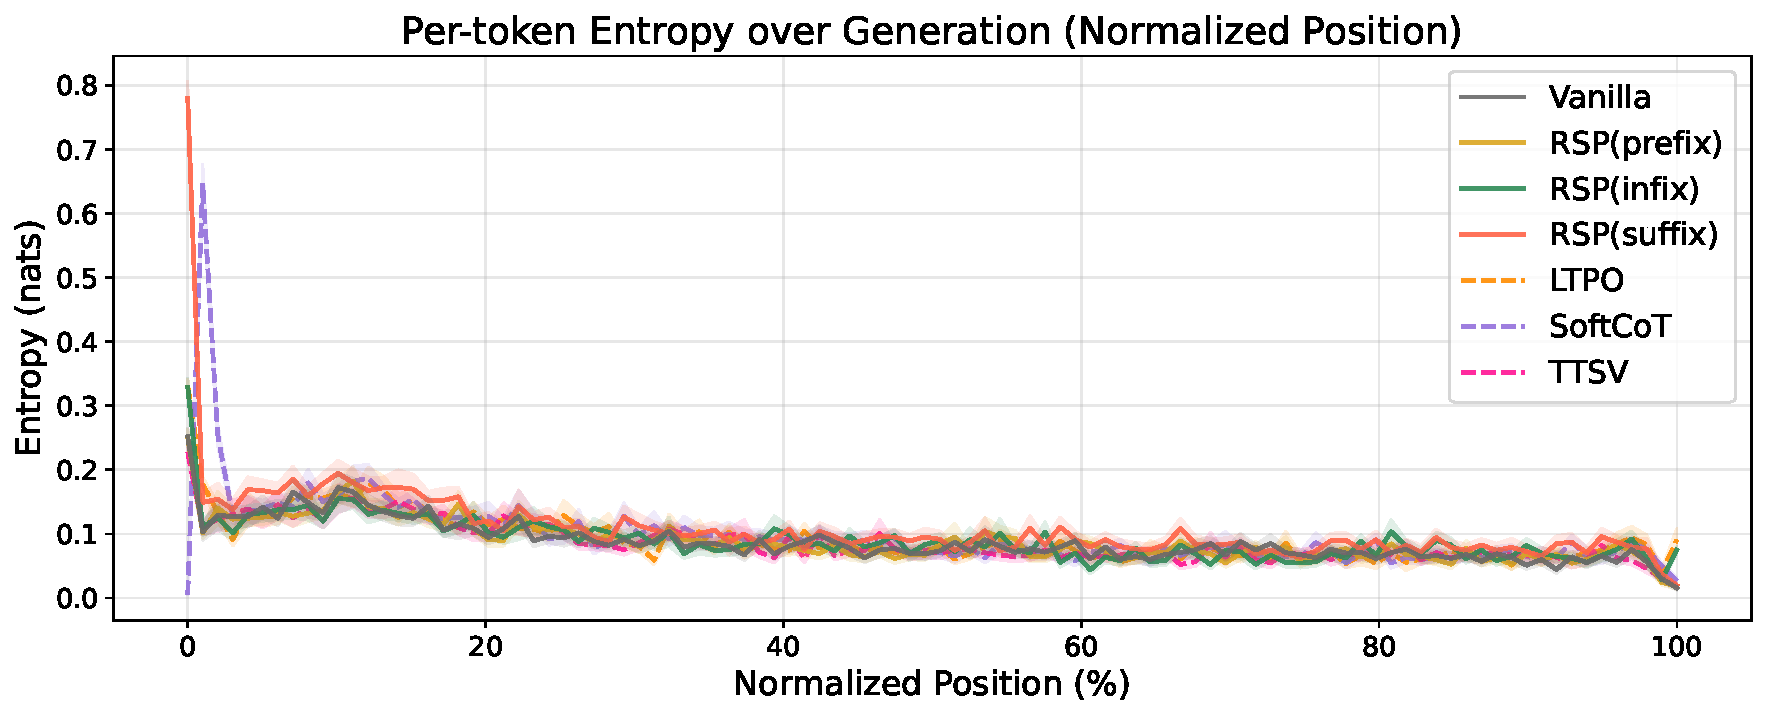
\includegraphics[width=0.85\textwidth]{img/entropy/full_entropy.pdf}\\[0.4em]
  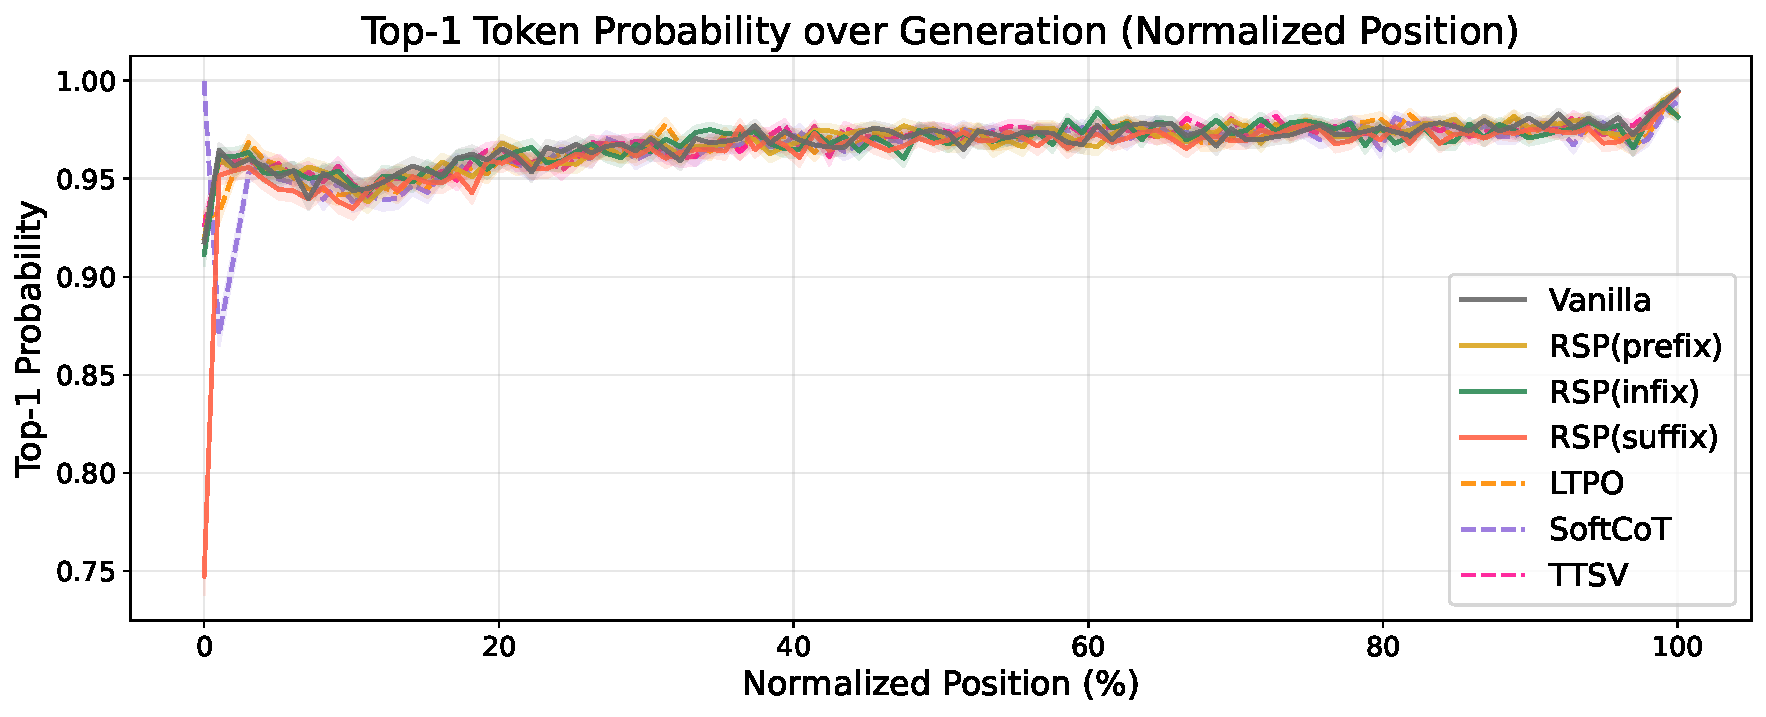
\includegraphics[width=0.85\textwidth]{img/entropy/full_top1prob.pdf}\\[0.4em]
  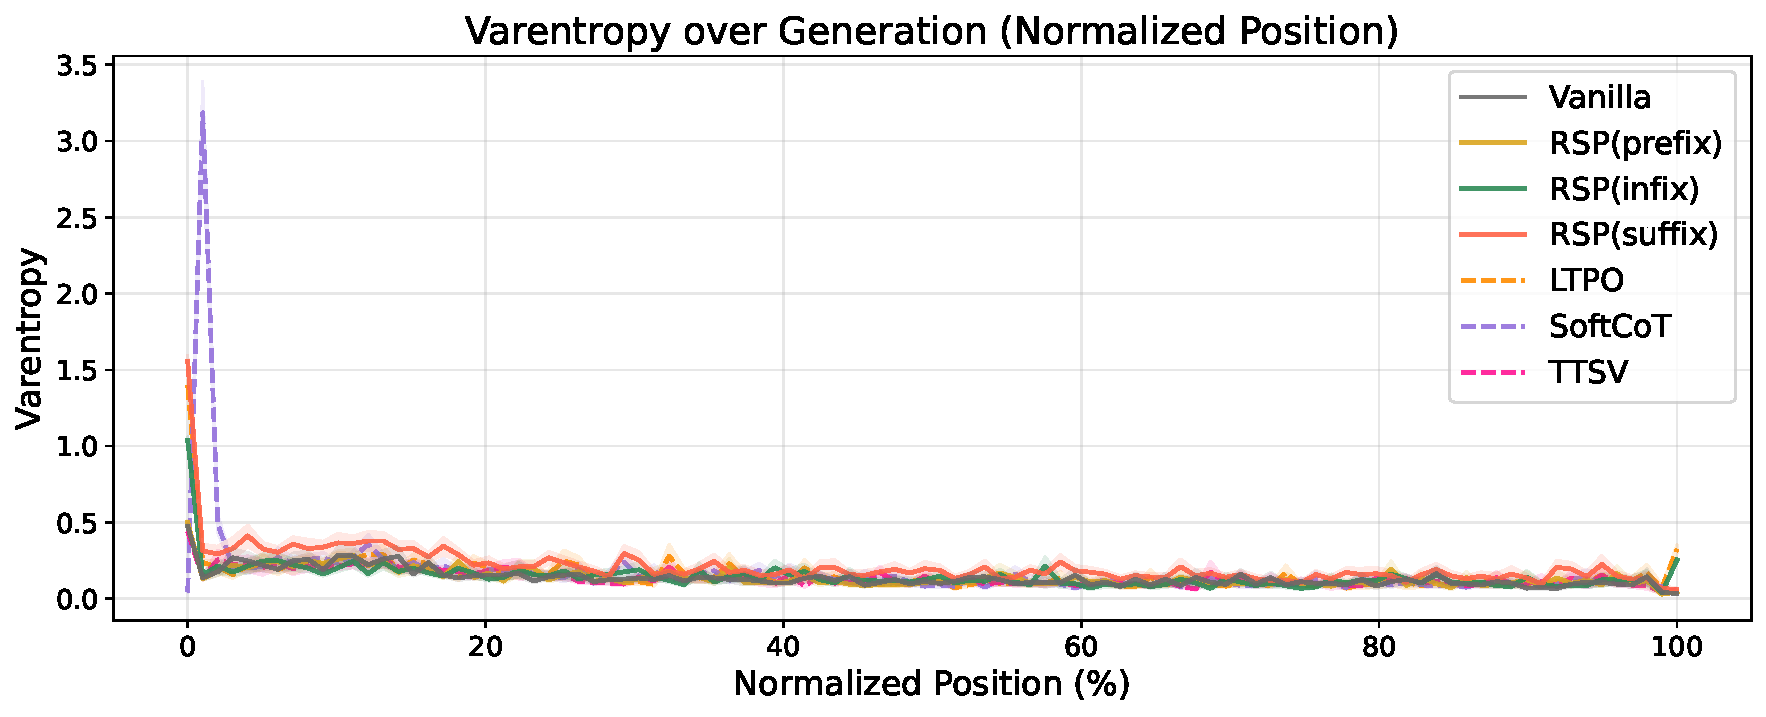
\includegraphics[width=0.85\textwidth]{img/entropy/full_varentropy.pdf}
  \caption{전체 정규화 생성 궤적(0--100\%)에서의 평균 entropy(위), top-1 probability(가운데), varentropy(아래). MATH-500 전체 평균이며, 음영은 $\pm$1 SEM을 뜻한다. 실선은 RSP 변형과 baseline, 점선은 기존 soft prompt 방법이다. 모든 방법은 초반 단계를 지나면 수렴한다.}
  \label{fig:app_full_entropy}
\end{figure}

\clearpage
\section{의미적 다양성에 대한 추가 분석}\label{app:semantic}

이 부록은 Section~\ref{sec:diversity}에서 보고한 의미적 다양성 결과를 보충한다. 더 넓은 문제 집합에 대해 문제별 t-SNE 도표를 함께 제시한다.

\begin{figure}[ht]
  \centering
  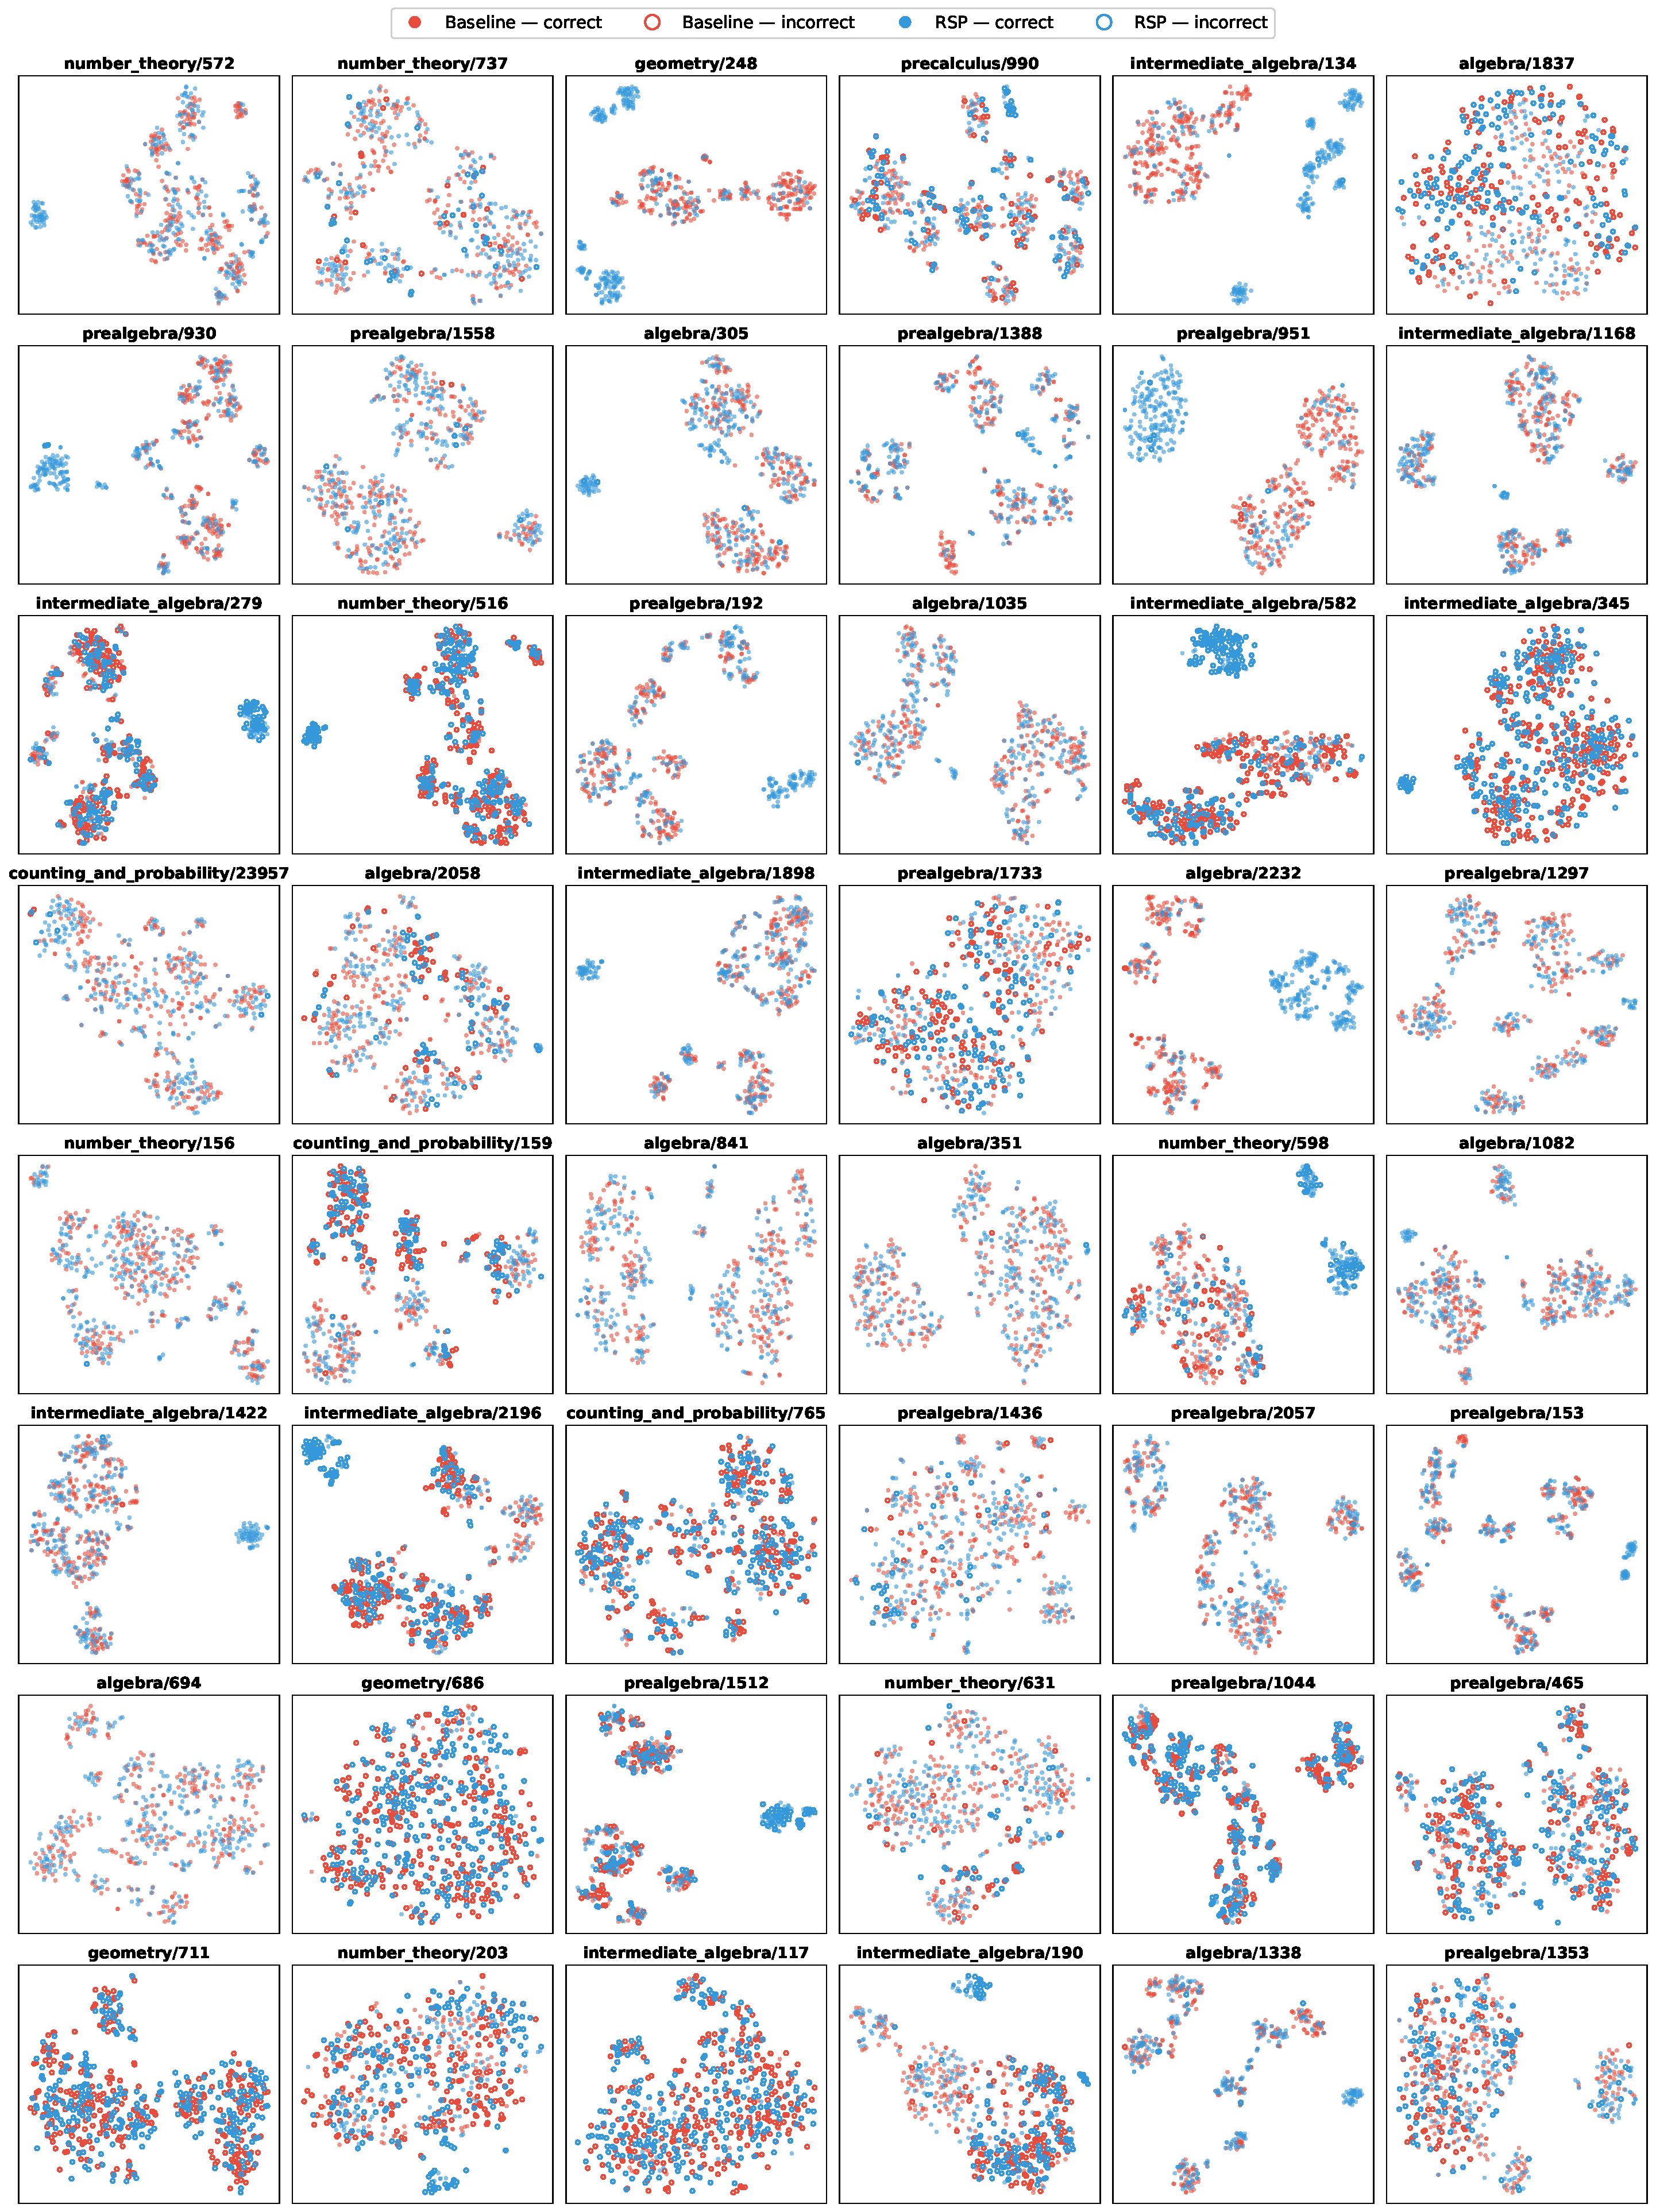
\includegraphics[width=\textwidth,height=0.75\textheight,keepaspectratio]{img/diversity/appendix_tsne_grid.pdf}
  \caption{평가한 64개 MATH-500 문제 중 48개에 대한 BGE-M3 임베딩의 t-SNE 투영(6$\times$8 격자). 각 subplot은 Qwen2.5-Math-1.5B-Instruct에서 $\tau=1.0$으로 생성한 baseline 300개(빨강)와 RSP suffix 300개(파랑)를 보여준다. 채워진 표식은 정답, 빈 표식은 오답이며, 제목은 \texttt{subject/problem\_id}를 뜻한다. 대부분의 문제에서 RSP 궤적은 여러 개의 분리된 영역으로 퍼지는 반면, baseline 샘플은 하나의 지배적 클러스터에 더 집중된다.}
  \label{fig:app_tsne_grid}
\end{figure}

\clearpage
\section{토큰 수준 분포 지표}\label{app:token_metrics}

이 부록은 Section~\ref{sec:diversity}의 토큰 수준 분석에 사용한 세 지표를 형식적으로 정의한다. $P_{\text{base}}$는 $\tau=1.0$에서의 baseline 다음 토큰 분포, $P_{\text{target}}$은 비교 대상 분포(예: $\tau=2.0$의 baseline, 또는 $\tau=1.0$의 RSP)라 하자. 모든 지표는 첫 생성 단계에서 저장한 logits로부터 해석적으로 계산한다.

\paragraph{Spearman 순위 상관.}
Spearman의 $\rho$는 두 분포의 토큰 순위 사이 Pearson 상관계수다.
\begin{equation}
\rho \;=\; \mathrm{Pearson}\!\left(\mathrm{rank}(P_{\text{target}}),\; \mathrm{rank}(P_{\text{base}})\right).
\end{equation}
Temperature scaling $P^{(\tau)} \propto P^{1/\tau}$는 엄격한 단조 변환이므로, 어떤 $\tau > 0$에서도 토큰 순서를 정확히 보존한다. 따라서 $\rho = 1$은 수학적 항등식이다. 그러므로 $\rho < 1$은 temperature scaling만으로는 만들 수 없는 순위 재조직이 일어났음을 뜻한다.

\paragraph{Top-$K$ 밖의 질량.}
$\mathrm{TopK}(P_{\text{base}})$를 $P_{\text{base}}$에서 확률이 가장 높은 $K$개 토큰의 집합이라 하자. 비교 대상 분포가 이 집합 \emph{밖에} 두는 확률 질량은
\begin{equation}
\mathrm{MassOutside}_K \;=\; 1 - \sum_{t \in \mathrm{TopK}(P_{\text{base}})} P_{\text{target}}(t).
\end{equation}
이 지표는 지지 집합 확장을 직접 측정한다. 즉 baseline의 선호 집합에 없던 토큰에 비교 대상이 얼마나 많은 확률을 배정하는지를 본다. 본문에 보고한 값은 $K = 10$을 사용했다.

\paragraph{Jensen--Shannon divergence.}
Kullback--Leibler divergence의 대칭적이고 bounded된 형태는 다음과 같다.
\begin{equation}
\mathrm{JS}(P, Q) \;=\; \tfrac{1}{2}\,\mathrm{KL}(P \,\|\, M) + \tfrac{1}{2}\,\mathrm{KL}(Q \,\|\, M), \qquad M = \tfrac{1}{2}(P + Q).
\end{equation}
로그는 밑이 2이므로 $\mathrm{JS} \in [0, 1]$이다. 저장한 top-100 바깥의 토큰에는 softmax 전에 sentinel logit($-10^9$)을 넣었는데, 본 설정에서는 top-5가 이미 확률 질량의 $99.9\%$ 이상을 덮기 때문에 이 근사는 무시 가능하다.

\clearpage
\section{무작위 프롬프트는 왜 의미적으로 중립적이고 방향적으로 포괄적인가}\label{app:why_random}

이 부록은 Section~\ref{sec:multipath}에서 사용한 주장을 형식화한다. 핵심은 무작위 프롬프트가 유용한 잠재 의미를 담고 있다는 것이 아니다. 더 약하고 정확한 주장은, 중심화한 뒤에는 어떤 미리 정한 의미 방향도 체계적으로 편들지 않으면서도, 고정된 분산 예산 아래 모든 방향을 덮을 수 있다는 것이다. 이는 언어학적 의미가 완전히 사라진다는 주장이 아니라, 섭동 방향의 기하학적 성질에 관한 명제다.

\subsection{의미적 중립성}

$\bar{h} \sim \mathcal{N}(0, \sigma^2 \mathbf{I}_d)$라 하고, $\bar{h}\neq 0$일 때 $\hat{h} := \bar{h}/\|\bar{h}\|$라 하자. 또한 $u_1,\dots,u_M \in \mathbb{S}^{d-1}$를 의미 anchor 방향을 나타내는 임의의 고정 단위벡터라 하자.

\begin{lemma}[의미적 중립성]\label{lem:semantic_neutrality_proof}\label{lem:semantic_neutrality}
보편 상수 $C$가 존재하여, 모든 $\delta \in (0,1)$에 대해
\[
\Pr\!\left[
\max_{r \in [M]} |\hat{h}^{\top} u_r|
\le
C \sqrt{\frac{\log(M/\delta)}{d}}
\right]
\ge 1-\delta.
\]
즉 등방성 가우시안 프롬프트의 정규화된 방향은, 고정된 유한 개의 의미 anchor 전체에 대해 높은 확률로 거의 직교한다.
\end{lemma}

\begin{proof}
각 고정 $u_r$에 대해 회전 불변성으로부터 $u_r^\top \bar{h} \sim \mathcal{N}(0,\sigma^2)$가 성립하므로,
\[
\Pr\big(|u_r^\top \bar{h}| \ge t\big) \le 2\exp\!\left(-\frac{t^2}{2\sigma^2}\right).
\]
$r \in [M]$ 전체에 대해 union bound를 적용하면
\[
\Pr\!\left[\max_{r \in [M]} |u_r^\top \bar{h}| \ge t\right]
\le
2M \exp\!\left(-\frac{t^2}{2\sigma^2}\right).
\]
한편 표준 chi-square concentration으로부터 보편 상수 $c>0$가 존재하여
\[
\Pr\!\left[\|\bar{h}\| \le \frac{\sigma \sqrt{d}}{2}\right]
\le
\exp(-cd)
\]
가 성립한다. 사건 $\|\bar{h}\| \ge \sigma\sqrt{d}/2$ 위에서는
\[
|\hat{h}^{\top} u_r|
=
\frac{|u_r^\top \bar{h}|}{\|\bar{h}\|}
\le
\frac{2 |u_r^\top \bar{h}|}{\sigma \sqrt{d}}.
\]
이제
\[
t = C' \sigma \sqrt{\log(M/\delta)}
\]
로 두고 $C'$를 충분히 큰 상수로 잡으면, 두 bound를 결합해
\[
\max_{r \in [M]} |\hat{h}^{\top} u_r|
\le
C \sqrt{\frac{\log(M/\delta)}{d}}
\]
가 적어도 $1-\delta$ 확률로 성립한다.
\end{proof}

토큰 임베딩과의 대비는 즉각적이다. $e_s \neq 0$를 고정된 토큰 임베딩이라 하고 $\hat{e}_s := e_s/\|e_s\|$라 하자. 이때 anchor 방향을 $u = \hat{e}_s$로 잡으면
\[
|\hat{e}_s^\top u| = 1.
\]
즉 토큰 프롬프트는 적어도 하나의 의미 방향과 최대 정렬을 이루지만, 등방성 무작위 프롬프트는 어떤 고정된 유한 집합의 의미 방향에도 거의 직교한다. 우리가 말하는 ``의미적 비개입성''은 바로 이 뜻이다. 토큰은 의미적 commitment를 주입하는 반면, 무작위 프롬프트는 의미적으로 특정 방향에 묶이지 않은 섭동으로 기능한다.

\subsection{Theorem~\ref{thm:minimax_directional_coverage} (미니맥스 방향 커버리지)의 증명}

본문에서 사용한 local linear logit surrogate에 직접 등장하는 양은 단위벡터 $b$에 대해 $b$ 방향의 1차 섭동 에너지 $\mathrm{Var}_{h\sim D}(b^\top h)=b^\top\Sigma_D b$이다. $\min_{\|b\|=1}b^\top\Sigma_D b = \lambda_{\min}(\Sigma_D)$이므로 최소 방향 분산은 정확히 $\lambda_{\min}(\Sigma_D)$이다.

\begin{proof}[Theorem~\ref{thm:minimax_directional_coverage}의 증명]
$\Sigma_D$의 고윳값을 $\lambda_1,\dots,\lambda_d$라 하면,
\[
\lambda_{\min}(\Sigma_D)
\le
\frac{1}{d}\sum_{m=1}^{d}\lambda_m
=
\frac{\mathrm{tr}(\Sigma_D)}{d}
\le
\frac{\rho^2}{d}.
\]
모든 고윳값이 같을 때, 즉 $\Sigma_D = (\rho^2/d)\mathbf{I}_d$일 때 그리고 그럴 때만 등호가 성립한다.
\end{proof}

이 정리는 등방성 무작위성의 장점을 형식화한다. RSP는 어떤 logit-sensitive 방향을 섭동해야 하는지 사전에 알지 못하므로, 고정된 분산 예산 아래에서 등방성 분포는 모든 방향에 대한 최악 경우 섭동량을 유일하게 최대화한다. 고정 토큰 프롬프트는 결정적 섭동이므로 $\Sigma_D=0$이고 $\lambda_{\min}=0$이며, 비등방 섭동은 항상 $\lambda_{\min}(\Sigma_D)<\rho^2/d$이므로 적어도 한 방향에서 등방 최적해보다 덜 탐색하게 된다.

\clearpage
\section{본문 이론 결과의 증명}\label{app:proofs}

% [본문 문단 5 메커니즘 1에 대한 증명]
% RSP perturbation term의 expectation, covariance, bias-to-variance ratio
\subsection{RSP가 유도하는 섭동의 성질}\label{app:rsp_noise}

본문 Eq.~\eqref{eq:decomp}의 분해 $\mathbf{x}_i^{(\ell+1)} = (1-w_{r,i}^{(\ell)})\tilde{\mathbf{x}}_i^{(\ell+1)} + \boldsymbol{\eta}_i^{(\ell)}$에서 무작위 기여 항 $\boldsymbol{\eta}_i^{(\ell)} = \sum_{j=1}^{L}\alpha_{i,n+j}^{(\ell)}\mathbf{v}_{r_j}^{(\ell)}$의 통계적 성질을 분석한다. 입력층의 RSP는 등방 가우시안이지만, layer $\ell$에서의 value vector $\mathbf{v}_{r_j}^{(\ell)}$는 attention, residual, LayerNorm, FFN, value projection을 차례로 통과한 결과이므로 일반적으로 등방 가우시안이 아니다. 따라서 layer 이후의 분석은 \emph{bounded second moment}만 가정한 형태로 약화하는 것이 안전하다.

\paragraph{조건부 기댓값과 상계.}
입력층 statistics에 의해 layer-별 mean·norm을
\[
m_v^{(\ell)} := \max_j \big\|\mathbb{E}[\mathbf{v}_{r_j}^{(\ell)}]\big\|,
\qquad
M_v^{(\ell)} := \max_j \mathbb{E}\big\|\mathbf{v}_{r_j}^{(\ell)}\big\|^2 \;<\; \infty
\]
라 두자(유한성은 implementation-side 가정으로 자연스럽다). 어텐션 가중치에 조건부로 두면
\begin{equation}
\bigl\|\mathbb{E}\!\left[\boldsymbol{\eta}_i^{(\ell)} \mid \alpha^{(\ell)}\right]\bigr\| \;\le\; w_{r,i}^{(\ell)} \, m_v^{(\ell)}.
\end{equation}
입력층($\ell=0$)에서는 등방 RSP에 대해 $m_v^{(0)} = |\mu_E|$이며, 항별 평균이 0에 가까운 임베딩 행렬에서 작아진다 — Table~\ref{tab:embed_stats} 참조.

\paragraph{조건부 disturbance energy(Lyapunov-style upper bound).}
$V_{\eta,i}^{(\ell)} := \mathbb{E}\big\|\boldsymbol{\eta}_i^{(\ell)}\big\|^2$로 두면, Cauchy-Schwarz와 $\sum_j \alpha_{i,n+j}^{(\ell)} = w_{r,i}^{(\ell)}$에서
\begin{equation}\label{eq:lyap_eta}
V_{\eta,i}^{(\ell)} \;\le\; M_v^{(\ell)}\,\bigl(w_{r,i}^{(\ell)}\bigr)^2.
\end{equation}
이는 ``RSP가 주입하는 disturbance energy의 상계가 $w_r^2$로 통제된다''는 Lyapunov-style stability 진술이다 — 정확한 등방성을 layer 이후에도 가정할 필요 없이, value norm의 second moment 유한성만으로 충분하다.

\paragraph{시퀀스 방향 attenuation 결합.}
Theorem~\ref{thm:decay}와 결합하면 \emph{같은 layer, 같은 query 위치, 같은 logit gap} 아래에서 $w_{r,i}^{(\ell)} = O(1/n)$이고, Eq.~\eqref{eq:lyap_eta}로부터 $V_{\eta,i}^{(\ell)} = O(1/n^2)$이다. layer 방향에 대한 단조 감소는 $M_v^{(\ell)}$, $\Delta_i^{(\ell)}$, hidden state geometry가 layer마다 달라지므로 일반적으로 보장되지 않는다 — 본문 Figure~\ref{fig:attention_mass}의 layer-축 감소는 이 정리의 직접 귀결이 아니라 deeper layer가 실제 토큰 evidence에 더 정렬되는 별개의 경험적 현상이다.

\paragraph{입력층 등방성의 의의.}
입력층에서는 RSP가 $\mathcal{N}(\mu_E\mathbf{1}_d, \sigma_E^2\mathbf{I}_d)$로 정의되므로, 중심화한 $\bar h$는 정확히 등방이고 모든 방향에 양의 밀도(full support)를 갖는다. Lemma~\ref{lem:semantic_neutrality}와 본문 §\ref{sec:multipath}의 결과는 이 입력층 등방성을 직접 사용하므로 layer 이후의 등방성 보존을 요구하지 않는다.

\begin{table}[ht]
\centering
\caption{임베딩 행렬 통계. 모든 모델에서 $|\mu_E|/\sigma_E < 0.02$이다.}
\label{tab:embed_stats}
\footnotesize
\renewcommand{\arraystretch}{0.9}
\begin{tabular}{lccc}
\toprule
\textbf{Model} & $\mu_E$ & $\sigma_E$ & $|\mu_E|/\sigma_E$ \\
\midrule
LLaMA-3.1-8B-Instruct & 0.00002 & 0.01057 & 0.002 \\
Qwen2.5-Math-7B-Instruct & $-$0.00002 & 0.01647 & 0.001 \\
Qwen2.5-Math-1.5B-Instruct & 0.00019 & 0.01585 & 0.012 \\
Qwen2.5-Math-7B & $-$0.00003 & 0.01842 & 0.001 \\
Qwen2.5-Math-1.5B & 0.00038 & 0.02990 & 0.013 \\
\bottomrule
\end{tabular}
\end{table}

\paragraph{함의.}
입력층에서 RSP가 $\mathcal{N}(\mu_E\mathbf{1}_d, \sigma_E^2\mathbf{I}_d)$로 시작하므로 입력층의 평균 항은 작지만, layer 이후의 $\mathbf{v}_{r_j}^{(\ell)}$는 일반적으로 \emph{bounded mean}만 가정한다. Eq.~\eqref{eq:lyap_eta}는 이 약한 가정 아래에서도 RSP 기여의 disturbance energy가 attention-local 수준에서 $w_{r,i}^{(\ell)}$로 통제됨을 보장한다 — 그 이상의 ``zero-mean noise처럼 동작한다''라는 강한 주장은 입력층에 한정된 해석이다.

\subsection{Eq.~\eqref{eq:decomp} 도출, Theorem~\ref{thm:decay}, Proposition~\ref{prop:lower_env}의 증명}

\paragraph{Eq.~\eqref{eq:decomp}의 도출.}
어텐션 출력 $\sum_{j=1}^{n+L}\alpha_{ij}^{(\ell)}\mathbf{v}_{ij}^{(\ell)}$를 실제 토큰 항과 RSP 토큰 항으로 가르고, 실제 항에서 정규화 인자 $1-w_{r,i}^{(\ell)} = \sum_{j=1}^n \alpha_{ij}^{(\ell)}$를 묶어 내면 본문 Eq.~\eqref{eq:decomp}가 그대로 나온다. softmax 정규화 항등식 $\sum_{j=1}^{n+L}\alpha_{ij}^{(\ell)}=1$ 외에는 어떤 근사도 사용하지 않는다.

\paragraph{Theorem~\ref{thm:decay} (upper envelope)의 증명.}
실제 토큰과 RSP 토큰의 scaled attention score를 각각 $s_j^{(\ell)} := (\mathbf{q}_i^{(\ell)})^\top\mathbf{k}_j^{(\ell)}/\sqrt d$ ($j\in[n]$), $s_{r_{j'}}^{(\ell)} := (\mathbf{q}_i^{(\ell)})^\top\mathbf{k}_{r_{j'}}^{(\ell)}/\sqrt d$ ($j'\in[L]$)라 하고, $s_{r,\max}^{(\ell)} := \max_{j'} s_{r_{j'}}^{(\ell)}$, $R^{(\ell)} := \sum_{j'=1}^L \exp(s_{r_{j'}}^{(\ell)})$로 둔다. 정방향 gap $\Delta_i^{(\ell)}/\sqrt d$의 정의에서 모든 $j\in[n]$에 대해 $s_j^{(\ell)} \ge s_{r,\max}^{(\ell)} + \Delta_i^{(\ell)}/\sqrt d$이고, max $\ge$ avg에서 $\exp(s_{r,\max}^{(\ell)}) \ge R^{(\ell)}/L$이다. 따라서 $\sum_{j=1}^n \exp(s_j^{(\ell)}) \ge n\,\exp(\Delta_i^{(\ell)}/\sqrt d)\cdot R^{(\ell)}/L$이고, softmax 정규화에서 $w_{r,i}^{(\ell)} = R^{(\ell)}/(\sum_j \exp(s_j^{(\ell)}) + R^{(\ell)}) \le L/(L+n\,\exp(\Delta_i^{(\ell)}/\sqrt d))$. $f(n) = L/(L+n\,\exp(\Delta_i^{(\ell)}/\sqrt d))$의 미분이 음수이므로 $n$에 대해 엄격 감소하고 $n\to\infty$에서 0으로 간다.

\paragraph{Proposition~\ref{prop:lower_env} (lower envelope)의 증명.}
대칭 도출이다. 역방향 gap $\Delta_i'^{(\ell)}/\sqrt d$의 정의에서 모든 $j\in[n]$에 대해 $s_j^{(\ell)} \le s_{r,\min}^{(\ell)} + \Delta_i'^{(\ell)}/\sqrt d$이며, min $\le$ avg에서 $\exp(s_{r,\min}^{(\ell)}) \le R^{(\ell)}/L$이다. 따라서 $\sum_{j=1}^n \exp(s_j^{(\ell)}) \le n\,\exp(\Delta_i'^{(\ell)}/\sqrt d)\cdot R^{(\ell)}/L$이고, $w_{r,i}^{(\ell)} = R^{(\ell)}/(\sum_j \exp(s_j^{(\ell)}) + R^{(\ell)}) \ge L/(L+n\,\exp(\Delta_i'^{(\ell)}/\sqrt d))$.

\subsection{Theorem~\ref{thm:decay}의 따름정리들}

위 envelope들로부터 두 가지 따름정리가 따른다.

\begin{corollary}[fixed-gap envelope의 시퀀스 방향 단조 감소]\label{cor:sequence_annealing}
$L$과 $\Delta_i^{(\ell)}$를 고정하면, 상계
\[
f(n)=\frac{L}{L+n\exp(\Delta_i^{(\ell)}/\sqrt{d})}
\]
는 실제 토큰 수 $n$에 대해 엄격히 감소한다. 따라서 \emph{동일한 logit gap을 유지한다는 가정 아래}, cache 성장만으로 그 gap과 양립 가능한 최대 RSP attention mass의 \emph{envelope}이 단조롭게 좁아진다.
\end{corollary}

\noindent 자기회귀 디코딩에서는 새 토큰이 생성될 때마다 query·key·hidden state가 갱신되어 $\Delta_i^{(\ell)}$도 step별로 변하므로, ``실현된 attention mass가 매 step 단조 감소한다''가 아니라 ``동일한 gap이 유지되는 한 가능한 최대 mass의 envelope이 단조 감소한다''가 정확한 진술이다.

\begin{proof}
$f(n)$을 $n$에 대해 미분하면
\[
f'(n)
=
-\frac{L\exp(\Delta_i^{(\ell)}/\sqrt{d})}{\left(L+n\exp(\Delta_i^{(\ell)}/\sqrt{d})\right)^2}
<
0.
\]
따라서 $f(n)$은 엄격히 감소한다.
\end{proof}

\begin{corollary}[고정 gap envelope 아래의 disturbance energy 감쇠]\label{cor:vanishing_perturbation}
$L$과 $\Delta_i^{(\ell)}$를 고정하고 $n\to\infty$이면 $w_{r,i}^{(\ell)} \to 0$이다. 본 절의 약화된 가정 하에서 attention-local disturbance energy는 다음과 같이 좁아진다.
\[
\bigl\|\mathbb{E}[\boldsymbol{\eta}_i^{(\ell)} \mid \alpha^{(\ell)}]\bigr\| \le m_v^{(\ell)}\,w_{r,i}^{(\ell)} \;\to\; 0,
\qquad
V_{\eta,i}^{(\ell)} \le M_v^{(\ell)}\,(w_{r,i}^{(\ell)})^2 \;\to\; 0.
\]
\end{corollary}

\begin{proof}
Corollary~\ref{cor:sequence_annealing}에서 $w_{r,i}^{(\ell)}\to 0$이고, 본 절의 평균·second-moment 상계 $m_v^{(\ell)}, M_v^{(\ell)} < \infty$를 곱하면 결과가 따른다.
\end{proof}

% [본문 Section 4.2 (Output Distribution Shift and Exploration) 에 대한 증명]
% autoregressive formulation, local linearization, Proposition 1/2 증명, trajectory-level implications
\subsection{출력 분포 이동에 대한 증명}

본문 §\ref{sec:multipath}는 surrogate 위 top-$K$ 진입 명제 (Proposition~\ref{prop:support_expansion})와 다중 경로 Pass@$N$ 누적 명제 (Proposition~\ref{prop:multi_path})를 다룬다. 보조적으로 쌍대 순위 무작위화 명제도 함께 둔다.

\subsubsection{자기회귀 정식화}

자기회귀 decoding에서 시퀀스 $y_{1:T}$의 결합 분포는
\[
\Pr(y_{1:T} \mid x) = \prod_{t=1}^T p(y_t \mid x, y_{<t}),
\]
로 분해된다. 각 단계는 prefix에 조건부인 분포로 결정되므로, RSP가 도입한 섭동은 단일한 전역 분포를 한 번에 바꾸는 것이 아니라 $p(y_t \mid x, y_{<t})$에 대한 일련의 국소 변화로 작동한다.

\subsubsection{RSP 하에서의 logits 국소 선형화}

중심화된 random soft prompt를 $\bar{h}$라 하자. 섭동된 logits를 $\bar{h}$의 함수로 보고 $\bar{h}=0$ 근방에서 국소 smoothness를 가정하면 $z_i(\bar{h}) = z_i + a_i^\top \bar{h} + O(\|\bar{h}\|^2)$이며, 여기서 $a_i := \nabla_{\bar h} z_i(0)$이다. 본문 §\ref{sec:multipath}와 같은 표기로 \emph{1차 surrogate}를 $z_i^{\mathrm{lin}}(\bar h) := z_i + a_i^\top \bar h$로 정의한다. 이 surrogate는 충분히 작은 $\|\bar{h}\|$에서 유효하며, transformer logits의 전역 모델이라기보다 섭동 방향을 설명하는 1차 근사다.

\subsubsection{명제 1의 증명 (확률적 순위화)}

\begin{proposition}[확률적 순위화]\label{prop:stochastic_ranking}
토큰 쌍 $(i,j)$ 중 $a_i \neq a_j$인 것이 존재하면, $0 < \Pr_{\bar{h}}(z_i^{\mathrm{lin}}(\bar{h}) > z_j^{\mathrm{lin}}(\bar{h})) < 1$이 성립한다.
\end{proposition}

\begin{proof}
$z_i^{\mathrm{lin}}(\bar{h}) - z_j^{\mathrm{lin}}(\bar{h}) = (z_i-z_j) + (a_i-a_j)^\top \bar{h}$이고, $b_{ij}:=a_i-a_j \neq 0$이며 $\bar{h} \sim \mathcal{N}(0,\sigma^2 I)$이면 $b_{ij}^\top \bar{h} \sim \mathcal{N}(0,\sigma^2 \|b_{ij}\|^2)$인 비퇴화 가우시안이다. 따라서 섭동된 logit 차이는 0의 양쪽에 모두 양의 확률 질량을 갖고, $0 < \Pr_{\bar{h}}(z_i^{\mathrm{lin}}(\bar{h}) > z_j^{\mathrm{lin}}(\bar{h})) < 1$이 성립한다.
\end{proof}

\subsubsection{명제 2의 증명 (지지 집합 확장)}

\begin{proposition}[지지 집합 확장]\label{prop:support_expansion}
어떤 토큰 $i$에 대해 진입 영역
\[
\mathcal{G}_{i,K} \;:=\; \bigl\{\bar h \in \mathbb{R}^d : \#\{j\neq i : z_j^{\mathrm{lin}}(\bar h) > z_i^{\mathrm{lin}}(\bar h)\} \le K-1\bigr\}
\]
이 비공집합 열린집합을 포함한다고 하자. centered RSP $\bar h$가 등방 가우시안에서 추첨되면 $\Pr_{\bar h}(\bar h \in \mathcal{G}_{i,K}) > 0$이 성립한다.
\end{proposition}

\begin{proof}
$\mathcal{G}_{i,K}$가 비공집합 열린집합 $U$를 포함한다고 하자. centered 등방 가우시안은 $\mathbb{R}^d$ 전역에서 엄밀히 양수인 밀도를 가지므로 모든 비공집합 열린집합에 양의 확률 측도를 부여한다. 따라서 $\Pr_{\bar h}(\bar h \in \mathcal{G}_{i,K}) \ge \Pr_{\bar h}(\bar h \in U) > 0$이다. 정의상 $\mathcal{G}_{i,K}$는 정확히 surrogate logit이 $i$를 top-$K$로 진입시키는 사건이다.

\smallskip
\noindent (충분조건 예시.) $i$가 어떤 baseline top-$K$ 부분집합 $S\subseteq J_K(s_t)$ ($|S|=K$)의 모든 원소를 엄격한 마진으로 앞서는 $\bar h_0$가 존재하면, surrogate의 연속성으로 $\bar h_0$ 주변 비공집합 열린집합이 $\mathcal{G}_{i,K}$에 포함된다 (각 부등식이 열린 half-space를 정의).
\end{proof}

\subsubsection{궤적 수준의 함의: 다중 경로 Pass@$N$}

자기회귀 생성은 조건부 분포를 단계별로 합성하므로, 초기 단계의 섭동이 전혀 다른 궤적으로 이어질 수 있다. 적어도 한 번 baseline top-$K$ 바깥 토큰을 포함하는 궤적의 집합을 $\mathcal{R}_{L,K}(x)$라 하자. 만약 RSP가 초기 단계에서 이런 토큰의 접근 가능성을 높인다면, 반복 샘플링에서 $\mathcal{R}_{L,K}(x)$에 속하는 궤적을 뽑을 확률도 증가한다. 핵심은 시간적 누적이다. 초반의 top-$K$ 진입 한 번이 다음 decoding state를 바꾸고, 그것이 다시 다음 후보 집합을 바꾸는 식으로 이어진다. 이를 형식적으로 모으면 다음 명제가 된다.

\begin{proposition}[다중 경로 Pass@$N$]\label{prop:multi_path}
문제 $x$를 고정하고 정답 궤적 집합 $\mathcal{T}^\star(x)$가 비어 있지 않다고 하자. baseline 정답 지시자를 $p_{\mathrm{base}}(x)\in\{0,1\}$이라 하고, $N$개의 독립적이고 새로운 RSP를 추첨하여 표본당 한 번씩 디코딩한다. \textbf{(M1)} 각 $n$에 대해, $n$번째 RSP 실행이 $\mathcal{T}^\star(x)$의 궤적을 만들 주변 확률이 적어도 $p_{\min}(x)>0$이고, \textbf{(M2)} $N$번의 RSP 실행이 상호 독립이라 가정하자. 그러면
\[
\Pr\!\big(\mathrm{Pass@}N\text{ on }x\big) \;\ge\; 1-(1-p_{\min}(x))^N \;\ge\; 1-\exp(-Np_{\min}(x)).
\]
\end{proposition}

증명은 (M2)에 의한 곱 분해와 (M1)에 의한 단조 하한으로 곧바로 이루어진다. (M1)은 과제 측 가정이며 메커니즘만으로는 유도되지 않는다. 본문 §\ref{sec:diversity}에서 이 가정의 경험적 흔적을 논의했다.

\clearpage
% ================================================================
\section{Attention Mass 분석}\label{app:attention_mass}
% ================================================================

이 부록은 Figure~\ref{fig:attention_mass}에 보고한 per-token attention mass를 형식화하고, reasoning span과 layer 축에 적용한 제외 기준을 명시한다. 500개의 MATH-500 문제 각각에 대해 새로운 RSP $\mathbf{H} \in \mathbb{R}^{L \times d}$를 $L = 10$으로 독립 샘플링했으므로, 보고한 heatmap은 문제 자체의 변동성과 RSP 벡터 변동성을 함께 평균한 결과다.

\subsection{토큰당 attention 질량}

각 문제에서 attention은 연결된 시퀀스 $[\text{prompt}; \mathbf{H}; \text{generation}]$ 위에서 측정하며, generation은 같은 모델이 동일한 RSP 주입 설정 아래 생성한 궤적이다. $\alpha^{(\ell, h)}_{i,j}$를 layer $\ell$, head $h$에서 query 위치 $i$가 key 위치 $j$로 보내는 post-softmax attention weight라고 하자. 이는 causal mask 아래에서 $\sum_j \alpha^{(\ell, h)}_{i,j} = 1$을 만족한다. 질문 토큰과 RSP 토큰의 인덱스 집합을 각각 $Q$, $R$라 하고 크기를 $|Q|$, $|R| = L$, head 수를 $H$라 하자. 이때 query $i$가 각 그룹으로 보내는 layer $\ell$의 per-token attention mass는
\begin{equation}
\mathrm{PTM}_{Q}[\ell, i] = \frac{1}{|Q| H} \sum_{h=1}^{H} \sum_{j \in Q} \alpha^{(\ell, h)}_{i,j},
\qquad
\mathrm{PTM}_{R}[\ell, i] = \frac{1}{|R| H} \sum_{h=1}^{H} \sum_{j \in R} \alpha^{(\ell, h)}_{i,j}.
\label{eq:per_token_mass}
\end{equation}
$|Q|$와 $|R|$로 나누는 정규화는 집합 크기 차이를 보정하므로, 두 양은 동일한 softmax 분모 아래에서 질문 토큰 또는 RSP 토큰 하나가 평균적으로 얼마나 많은 attention을 받는지를 나타낸다. 따라서 질문 토큰은 시퀀스 길이 효과를 흡수하는 크기 보정 baseline 역할을 한다.

\subsection{Heatmap 집계}

Layer 인덱스와 reasoning position 인덱스를 각각 동일 크기의 다섯 구간 $\{B_L^{(b)}\}_{b=1}^{5}$, $\{B_P^{(b)}\}_{b=1}^{5}$로 나눈다. 샘플 $s$와 목표 집합 $\bullet \in \{Q, R\}$에 대해 셀 $(b_L, b_P)$의 값은
\begin{equation}
M^{(s)}_{\bullet}[b_L, b_P] = \frac{1}{|B_L^{(b_L)}| \cdot |B_P^{(b_P)}|} \sum_{\ell \in B_L^{(b_L)}} \sum_{i \in B_P^{(b_P)}} \mathrm{PTM}_{\bullet}[\ell, i].
\label{eq:binned_mass}
\end{equation}
Figure~\ref{fig:attention_mass}는 Eq.~\eqref{eq:binned_mass}를 500개의 유효 샘플에 대해 평균한 결과를 보고한다.

\subsection{\texttt{\textbackslash boxed\{\ldots\}} 구간 제외}

Reasoning position 범위는 마지막 \texttt{\textbackslash boxed\{\ldots\}} 구간이 시작되기 직전에 끝나도록 잡는다. Chain-of-thought 출력은 \textit{text}(내용)와 \textit{pattern}(형식) 성분으로 나뉘며, 이 둘은 downstream 성능에 독립적으로 기여할 수 있다 \citep{madaan2022text}. \texttt{\textbackslash boxed\{\ldots\}} 래퍼는 전형적인 pattern 성분이다. 이는 추론을 더 전개하기보다는 답 형식을 마무리하는 짧고 정형화된 span이기 때문이다. 이 구간을 포함하면 reasoning dynamics와 무관한 template-driven attention signature가 섞이게 된다.

\subsection{마지막 두 레이어 제외}

Layer 축에서는 마지막 두 transformer layer도 제외한다. 이는 우리 설정에만 특수한 것이 아니라, late layer의 두 가지 잘 알려진 성질에서 비롯된다.

\paragraph{출력 투영 특화.}
마지막 레이어 근방의 hidden state는 vocabulary logits와 거의 선형 관계를 이루므로, 표현을 바꾸는 블록이라기보다 점진적 선형 readout으로 기능한다 \citep{belrose2023eliciting}. 같은 맥락에서 late-layer feed-forward module도 출력 분포를 조정하는 메커니즘으로 해석되어 왔다 \citep{geva2021transformer}. 따라서 이 레이어들의 attention은 reasoning computation보다 output formation을 더 강하게 반영한다.

\paragraph{Register-token 가설.}
Vision Transformer에서 정보가 거의 없는 patch token은 deeper layer에서 attention을 흡수하는 \textit{register}로 재활용될 수 있음이 알려져 있다 \citep{darcet2023vision}. RSP 역시 사전학습된 의미를 갖지 않는 연속 토큰이라는 점에서 유사한 성질을 가지므로, late transformer layer에서 비슷한 재활용이 일어날 가능성을 배제할 수 없다. 마지막 두 레이어를 제외하면 이런 register 유도 교란이 reasoning-phase 신호를 오염시키는 일을 막을 수 있다.

위의 두 근거는 late layer에서 나타나는 잘 알려진 현상, 즉 선형 readout과 잠재적 register 재활용이 reasoning-phase dynamics와 직교하는 attention signature를 만들 수 있음을 뜻한다. 마지막 두 레이어를 제거하는 것은 모델 특이적 tuning이 아니라 문헌에 근거한 원칙적 제외에 해당하며, 본문에서 강조한 \emph{시퀀스 방향(autoregressive position) attenuation}은 이 제외 없이 모든 레이어를 포함했을 때에도 동일하게 관찰된다 — Theorem~\ref{thm:decay}이 직접 보장하는 것은 sequence-direction attenuation이지 layer-direction monotonicity가 아니므로, 마지막 두 레이어를 포함시키더라도 본문 claim에 변화는 없다.

\subsection{추가적인 suffix heatmap}

Figure~\ref{fig:app_attention_additional}는 suffix 주입에서 Qwen2.5-Math-1.5B-Instruct와 LLaMA-3.1-8B-Instruct에 대해 동일한 per-token RSP attention 분석을 보고한다. 앞서 설명한 late-layer 이유 때문에 모든 셀에서 패턴이 완전히 동일하게 일반화되지는 않지만, 두 모델 모두에서 \emph{시퀀스 방향(가로축)의 단조 감소}는 §\ref{sec:converge}의 cache-growth upper envelope가 예측한 것과 일치한다. layer 축(세로)의 추가 감소는 별개의 경험적 sharpening 현상으로, Theorem~\ref{thm:decay}만으로 직접 따라오는 결과는 아니다.

\begin{figure}[ht]
  \centering
  \begin{subfigure}[b]{\textwidth}
    \centering
    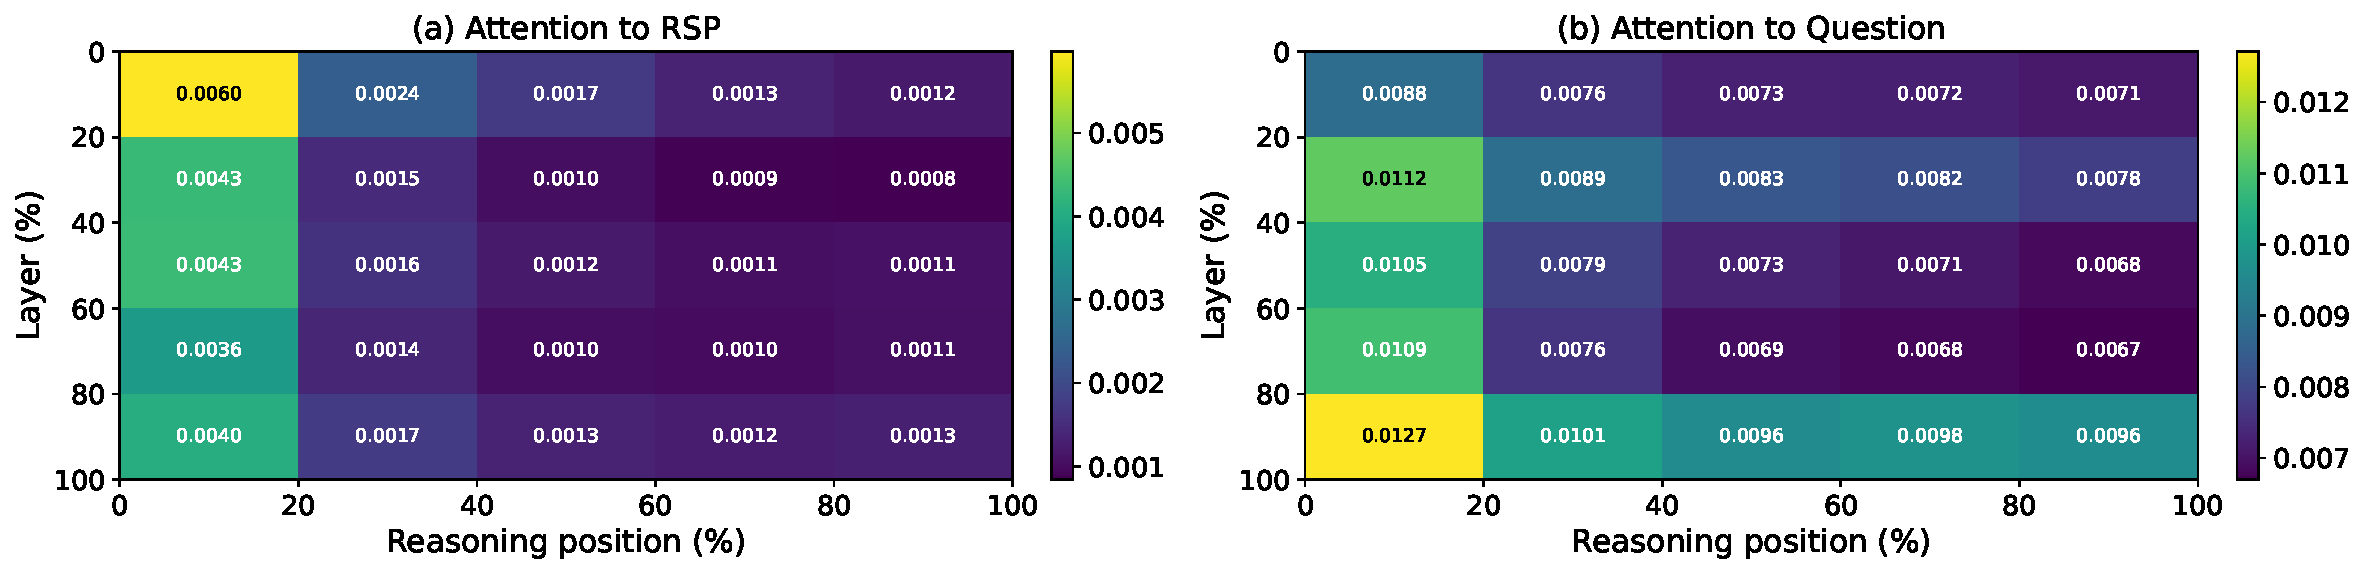
\includegraphics[width=\textwidth]{img/attention/heatmap_qwen1.5b_suffix.pdf}
    \caption{Qwen2.5-Math-1.5B-Instruct, suffix}
  \end{subfigure}
  \\[0.5em]
  \begin{subfigure}[b]{\textwidth}
    \centering
    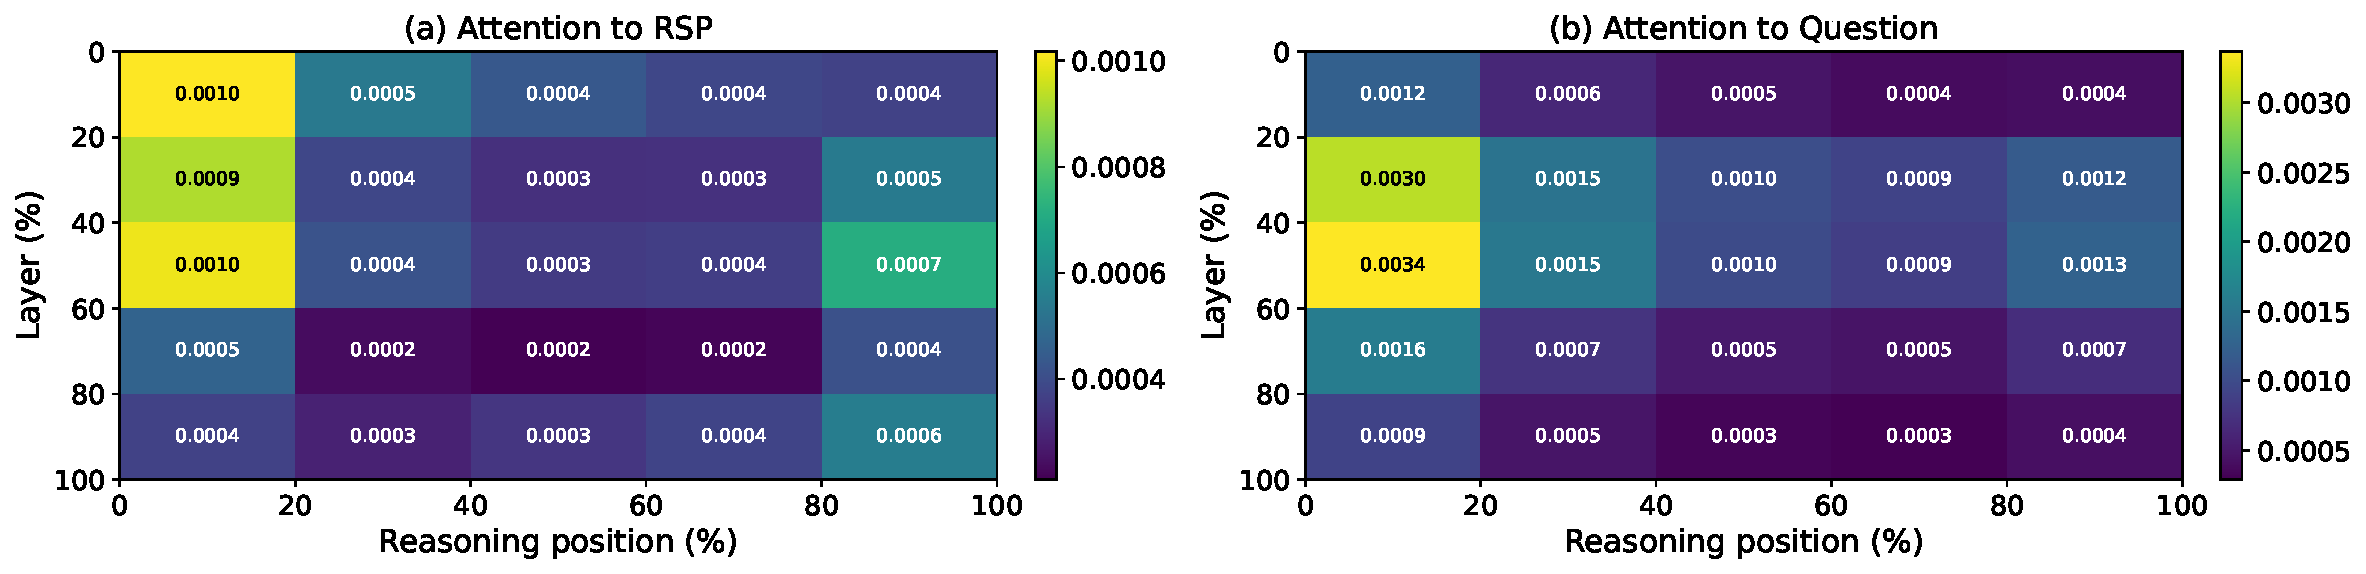
\includegraphics[width=\textwidth]{img/attention/heatmap_llama8b_suffix.pdf}
    \caption{LLaMA-3.1-8B-Instruct, suffix}
  \end{subfigure}
  \caption{나머지 두 모델(각각 500개 MATH-500 샘플)에서 suffix 주입 시 측정한 per-token RSP attention mass. 축과 전처리는 Figure~\ref{fig:attention_mass}와 동일하다. x축은 다섯 분위로 나눈 reasoning position, y축은 다섯 분위로 나눈 layer depth(위가 얕은 층), 색은 RSP 토큰에 할당된 per-token attention의 500샘플 평균을 뜻한다. \texttt{\textbackslash boxed\{\}} 구간 내부 토큰과 마지막 두 레이어는 제외했다.}
  \label{fig:app_attention_additional}
\end{figure}

\clearpage
% ================================================================
\section{GRPO 정식화}\label{app:grpo}
% ================================================================

주어진 프롬프트 $q$에 대해, behavior policy $\pi_{\theta_{\text{old}}}$는 보상 $\{R_i\}_{i=1}^G$를 갖는 응답 집합 $\{o_i\}_{i=1}^G$를 샘플링한다. 각 응답의 advantage는 그룹 수준 보상을 정규화해 계산한다.
\begin{equation}
  \hat{A}_{i,t} = \frac{R_i - \text{mean}(\{R_i\}_{i=1}^G)}{\text{std}(\{R_i\}_{i=1}^G)}.
\end{equation}
정책은 KL penalty가 포함된 clipped objective로 업데이트한다.
\begin{equation}
  \mathcal{J}_{\text{GRPO}}(\theta) = \mathbb{E} \left[ \frac{1}{G} \sum_{i=1}^{G} \frac{1}{|o_i|} \sum_{t=1}^{|o_i|} \left( \min\left( r_{i,t} \hat{A}_{i,t},\; \text{clip}(r_{i,t}, 1\!-\!\varepsilon, 1\!+\!\varepsilon)\, \hat{A}_{i,t} \right) - \beta D_{\text{KL}}(\pi_\theta \| \pi_{\text{ref}}) \right) \right],
\end{equation}
여기서 $r_{i,t} = \pi_\theta(o_{i,t} \mid q, o_{i,<t}) / \pi_{\theta_{\text{old}}}(o_{i,t} \mid q, o_{i,<t})$는 importance sampling ratio이고, $\varepsilon$는 clipping 범위, $\beta$는 reference policy $\pi_{\text{ref}}$에 대한 KL penalty 세기를 조절한다.

\clearpage
% ================================================================
\section{광범위한 영향}\label{app:broader_impacts}
% ================================================================

본 연구는 무작위 임베딩 주입이 대형 언어 모델의 추론 행동에 어떤 영향을 주는지에 대한 실험적·이론적 분석을 제공한다. 기여의 성격은 주로 기초 연구에 가깝지만, GRPO와 같은 강화학습 기반 추론 모델 후속학습에는 잠재적 함의를 가진다.

\paragraph{긍정적 영향.}
RSP가 유도하는 궤적 다양성은 group-relative advantage estimation 안에서 더 풍부한 학습 신호를 제공함으로써, RL 기반 LLM 후속학습의 sample efficiency를 높일 수 있다. 이는 reasoning 중심 fine-tuning과 alignment에 필요한 계산 비용을 줄여, 자원이 제한된 연구 그룹에도 관련 방법을 더 접근 가능하게 만들 수 있다.

\paragraph{잠재적 우려.}
LLM의 유효 출력 지지 집합을 넓히는 방법은 바람직한 대안적 추론 경로뿐 아니라, 바람직하지 않거나 분포 밖에 있는 출력의 도달 가능성도 함께 높일 수 있다. 따라서 RSP를 실제 시스템에 적용할 때는 이를 독립적인 다양성 원천으로만 보지 말고, 기존의 안전 필터링 및 alignment 메커니즘과 함께 사용해야 한다.

\paragraph{영향 범위의 한계.}
본 연구는 새로운 모델이나 데이터셋을 배포하기보다 분석을 제공하는 데 초점을 두므로, 직접적인 사회적 영향은 제한적이다. 여기서 논의한 더 넓은 함의는 RSP가 실제 학습 파이프라인에 통합되는 향후 연구가 이루어질 때에만 현실화될 수 있다.


\end{document}
